\documentclass[11pt,a4paper]{article}

\usepackage[utf8]{inputenc}
\usepackage[T1]{fontenc}
\usepackage{lmodern}
\usepackage[portuguese]{babel}
\usepackage{graphicx}
\usepackage{amsmath}
\usepackage{amsfonts}
\usepackage{amssymb}
\usepackage{float}
\usepackage{caption}
\usepackage{subcaption}
\usepackage{xcolor}
\usepackage{colortbl}
\usepackage{fancyhdr}
\usepackage{geometry}
\usepackage{titlesec}
\usepackage{booktabs}
\usepackage{array}
\usepackage{enumitem}
\usepackage{tikz}
\usetikzlibrary{shapes.geometric, positioning}
\usepackage[hidelinks]{hyperref}

\definecolor{headercolor}{HTML}{b11116}
\definecolor{secondarycolor}{HTML}{3a5461}

\geometry{
    a4paper,
    top=2.8cm,
    bottom=2.5cm,
    left=2.5cm,
    right=2.5cm,
    headheight=1.2cm,
    headsep=0.5cm
}

\pagestyle{fancy}
\fancyhf{}
\renewcommand{\headrulewidth}{0pt}
\renewcommand{\footrulewidth}{0.5pt}

\fancyhead[L]{%
    \begin{tikzpicture}[remember picture, overlay]
        \fill[headercolor] (current page.north west) rectangle ([yshift=-1.2cm]current page.north east);
        \node[anchor=west, inner sep=0pt] at ([xshift=1cm, yshift=-0.6cm]current page.north west)
            {
\includegraphics[height=0.8cm]{imgs/base/fatec-rgt.png}};
        \node[anchor=east, inner sep=0pt] at ([xshift=-1cm, yshift=-0.6cm]current page.north east)
            {
\includegraphics[height=0.9cm]{imgs/base/cps-logo.png}};
        \node[anchor=east, inner sep=0pt] at ([xshift=-2.8cm, yshift=-0.6cm]current page.north east)
            {
\includegraphics[height=1.05cm]{imgs/base/governo-sp-secretaria-logo.png}};
    \end{tikzpicture}
}

\fancyfoot[L]{\footnotesize\textcolor{secondarycolor}{Faculdade de Tecnologia do Estado de São Paulo\\ fatecregistro.cps.sp.gov.br}}
\fancyfoot[R]{\thepage}

\titleformat{\section}
    {\normalfont\large\bfseries\color{secondarycolor}}
    {\thesection}{1em}{}

\titleformat{\subsection}
    {\normalfont\normalsize\bfseries\color{secondarycolor}}
    {\thesubsection}{1em}{}

\begin{document}

\begin{titlepage}
    \centering
    \begin{tikzpicture}[remember picture, overlay]
        \fill[headercolor] (current page.north west) rectangle ([yshift=-1.2cm]current page.north east);
        \node[anchor=west, inner sep=0pt] at ([xshift=1cm, yshift=-0.6cm]current page.north west)
            {
\includegraphics[height=0.8cm]{imgs/base/fatec-rgt.png}};
        \node[anchor=east, inner sep=0pt] at ([xshift=-1cm, yshift=-0.6cm]current page.north east)
            {
\includegraphics[height=0.9cm]{imgs/base/cps-logo.png}};
        \node[anchor=east, inner sep=0pt] at ([xshift=-2.8cm, yshift=-0.6cm]current page.north east)
            {
\includegraphics[height=1.05cm]{imgs/base/governo-sp-secretaria-logo.png}};
    \end{tikzpicture}

    \vspace*{3.5cm}
    {\normalsize FACULDADE DE TECNOLOGIA DO ESTADO DE SÃO PAULO\par}
    \vspace{0.5cm}
    {\normalsize DESENVOLVIMENTO DE SOFTWARE MULTIPLATAFORMA\par}
    \vspace{4cm}
    {\normalsize ARTEFATOS DO PROJETO DE SOFTWARE\par}
    \vspace{0.3cm}
    {\normalsize Sistema Educacional de Baixo Custo com Realidade Aumentada para o Ensino de Montagem de Hardware\par}
    \vspace{3cm}
    {\normalsize
    Éric Pinheiro Abrahão Leandro\\
    Lucas do Nascimento Miura\\
    Luiz Ricardo Wandenkolk Medina\\
    Pedro Henrique da Silva
    }
    \vfill
    {\small Registro -- SP\\2026}
\end{titlepage}

\pagestyle{fancy}
\tableofcontents
\newpage

\section{CANVAS: Modelo de Negócio e Estratégia}
O Business Model Canvas é uma ferramenta visual utilizada para representar os principais elementos do modelo de negócio do SAVIT, incluindo proposta de valor, público-alvo, canais, recursos, atividades, parcerias, custos e fontes de receita.

\begin{figure}[H]
\centering
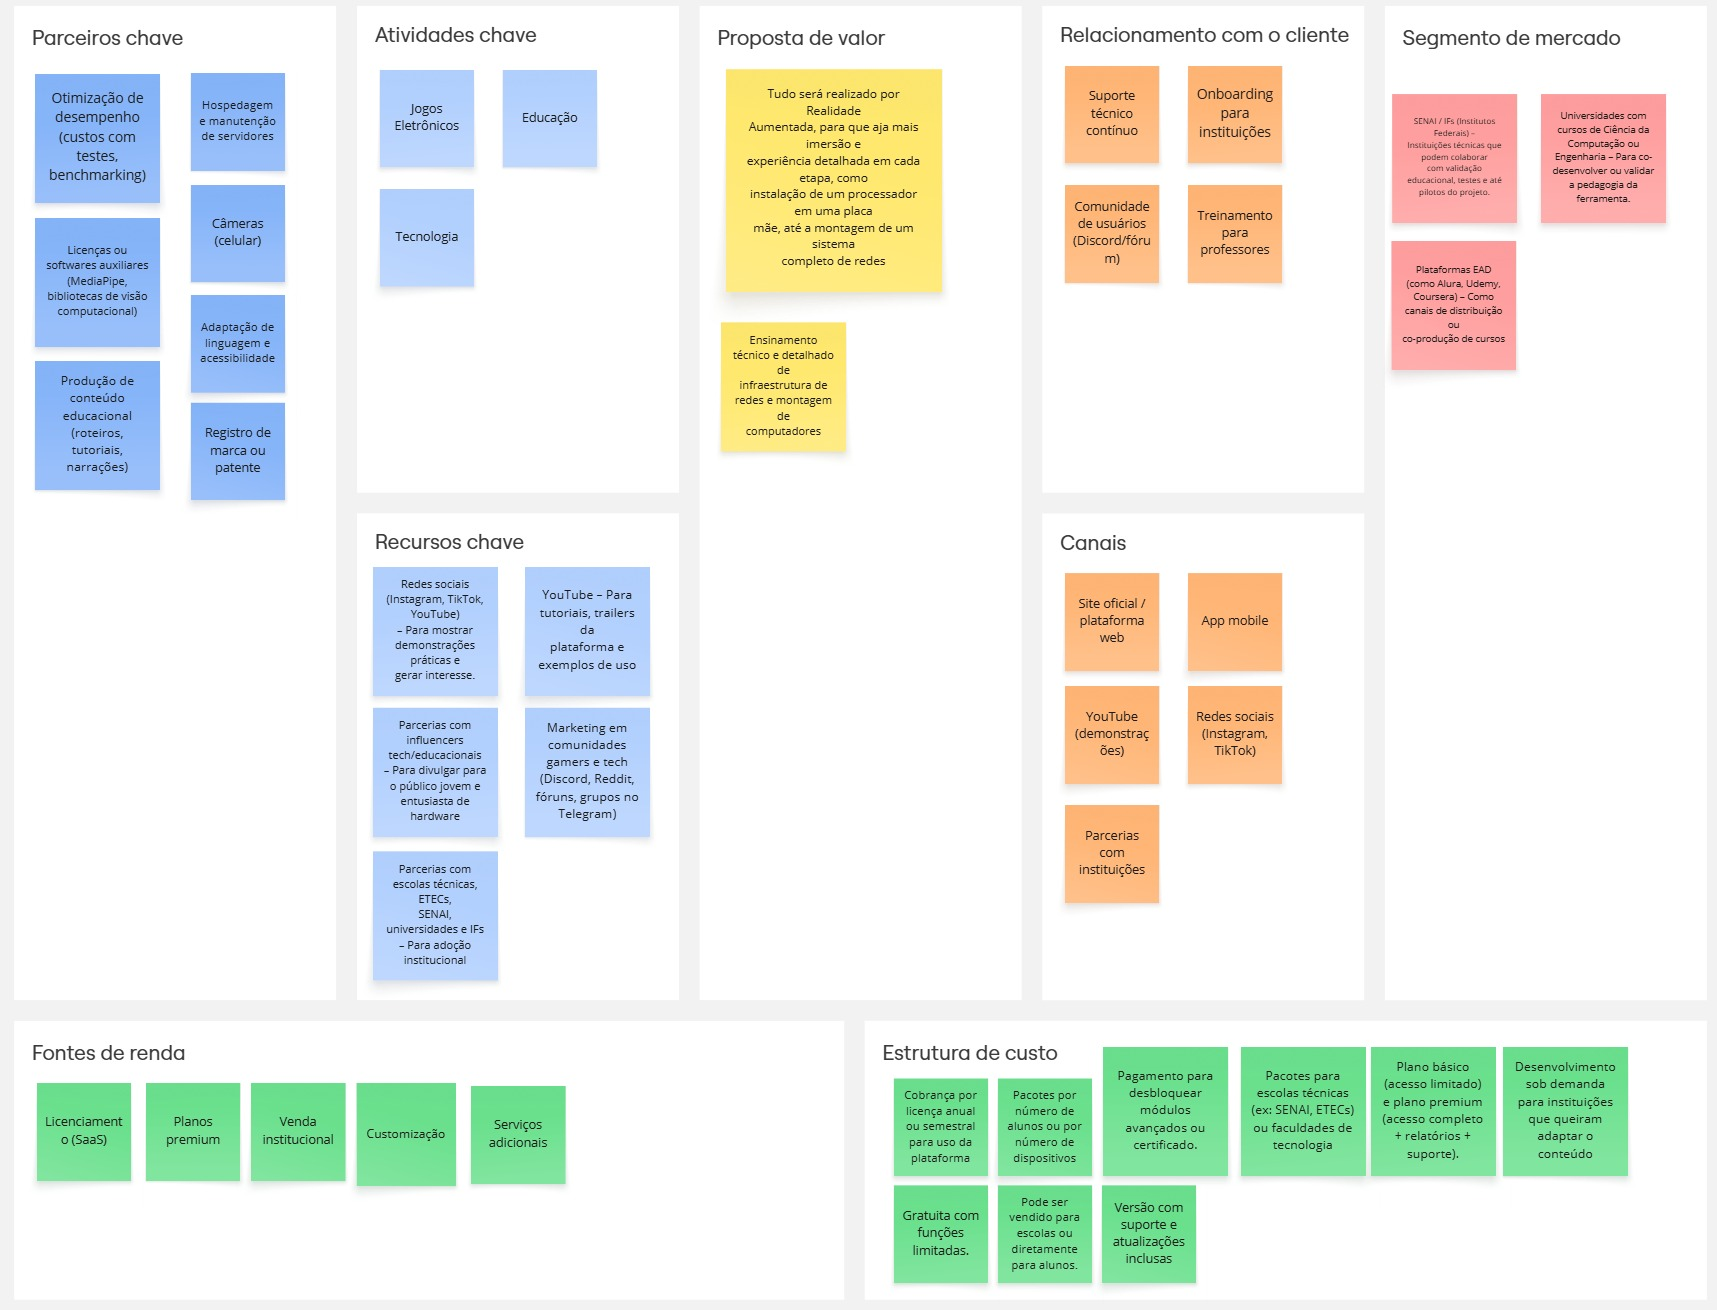
\includegraphics[width=\textwidth]{imgs/canvas-savit.png}
\caption{Business Model Canvas do projeto SAVIT.}
\label{fig:canvas}
\end{figure}

\section{SWOT: Análise Estratégica}
A análise SWOT identifica fatores internos e externos que podem influenciar o desenvolvimento e a utilização do SAVIT. A ferramenta considera forças, fraquezas, oportunidades e ameaças relacionadas à proposta de ensino de montagem de hardware com realidade aumentada.

\begin{figure}[H]
\centering
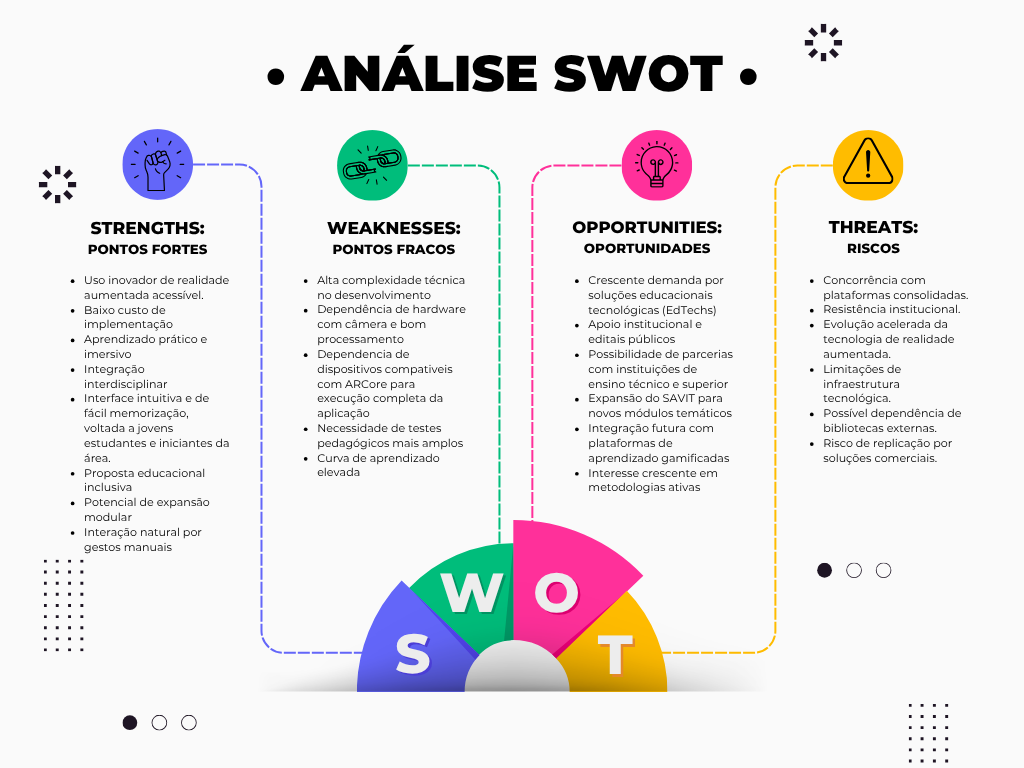
\includegraphics[width=\textwidth]{imgs/swot-savit.png}
\caption{Análise SWOT do projeto SAVIT.}
\label{fig:swot}
\end{figure}

\section{Metodologia do Projeto}
A metodologia de desenvolvimento adotada no SAVIT abrange desde o levantamento de problemas e pesquisa de campo preliminar até o planejamento, criação de assets 3D, desenvolvimento AR na Unity, tracking de mãos e testes.

\begin{figure}[H]
\centering
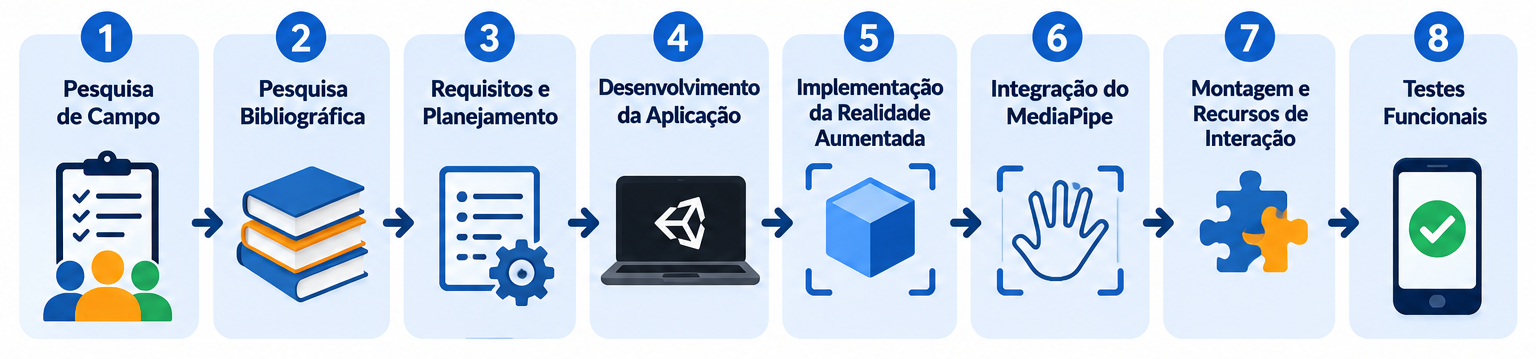
\includegraphics[width=\textwidth]{imgs/metodologia-savit.png}
\caption{Metodologia de desenvolvimento do projeto SAVIT.}
\label{fig:metodologia}
\end{figure}

\section{UX/UI: Design de Interface e Experiência do Usuário}
Esta seção apresenta os artefatos de interface do usuário e capturas reais da aplicação móvel em execução em dispositivo Android.

\subsection{Paleta de cores}
A Tabela~\ref{tab:paleta} apresenta as cores definidas para a identidade visual do projeto.

\begin{table}[H]
\centering
\caption{Paleta de cores do projeto.}
\label{tab:paleta}
\begin{tabular}{|l|c|l|l|}
\hline
\textbf{Elemento} & \textbf{Cor} & \textbf{Código HEX} & \textbf{Uso} \\
\hline
Primária & \colorbox[HTML]{151599}{\phantom{AAA}} & \#151599 & Botões principais e destaques \\
Secundária & \colorbox[HTML]{FB00FF}{\phantom{AAA}} & \#FB00FF & Títulos e elementos secundários \\
Fundo & \colorbox[HTML]{000000}{\phantom{AAA}} & \#000000 & Fundo padrão \\
Texto & \colorbox[HTML]{FFFFFF}{\phantom{AAA}} & \#FFFFFF & Texto principal \\
Sucesso & \colorbox[HTML]{28a745}{\phantom{AAA}} & \#28a745 & Mensagens de sucesso \\
Erro & \colorbox[HTML]{dc3545}{\color{white}\phantom{AAA}} & \#dc3545 & Mensagens de erro \\
\hline
\end{tabular}
\end{table}

\subsection{Personas}
As personas ajudam a entender as necessidades, limitações e objetivos dos principais usuários do SAVIT.

\begin{figure}[H]
\centering
\begin{subfigure}[t]{0.48\textwidth}
    \centering
    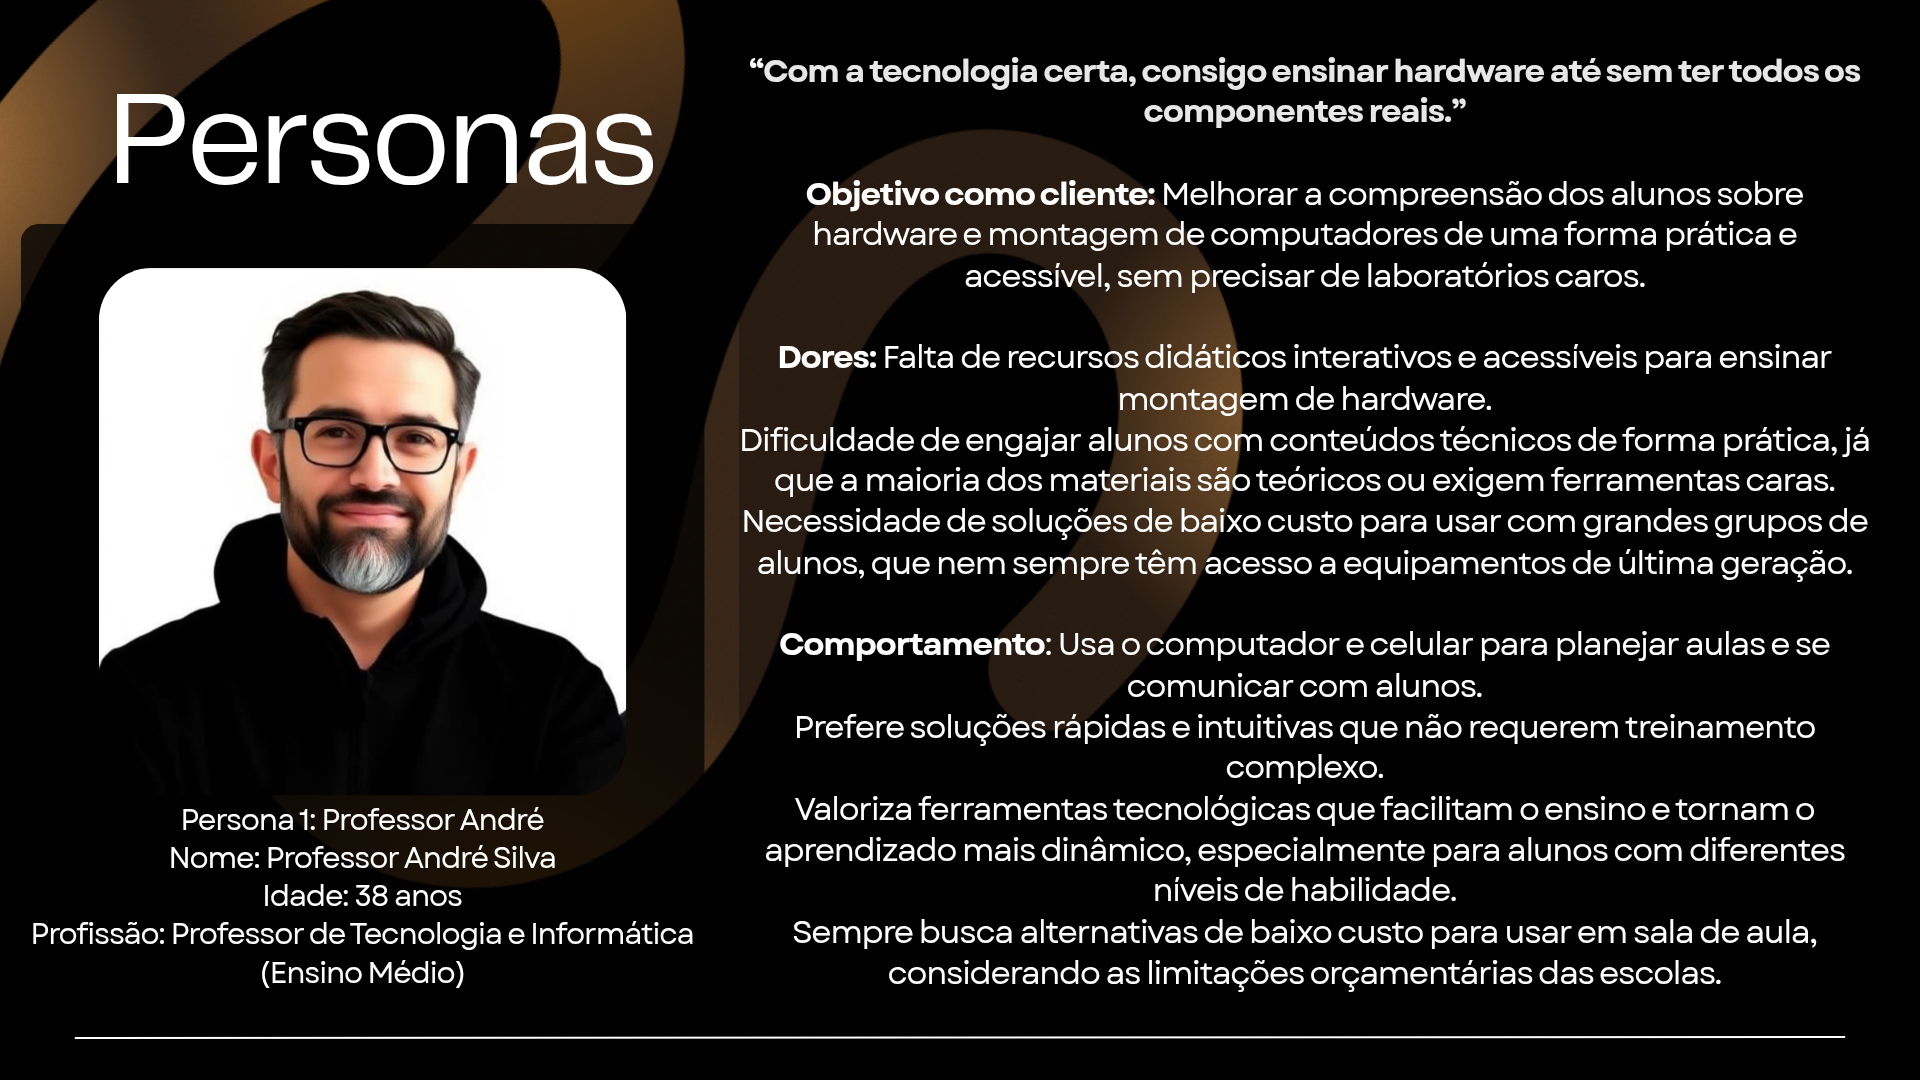
\includegraphics[width=\textwidth]{imgs/briefing_persona01.png}
    \caption{Persona 1: Professor André Silva.}
    \label{fig:persona01}
\end{subfigure}
\hfill
\begin{subfigure}[t]{0.48\textwidth}
    \centering
    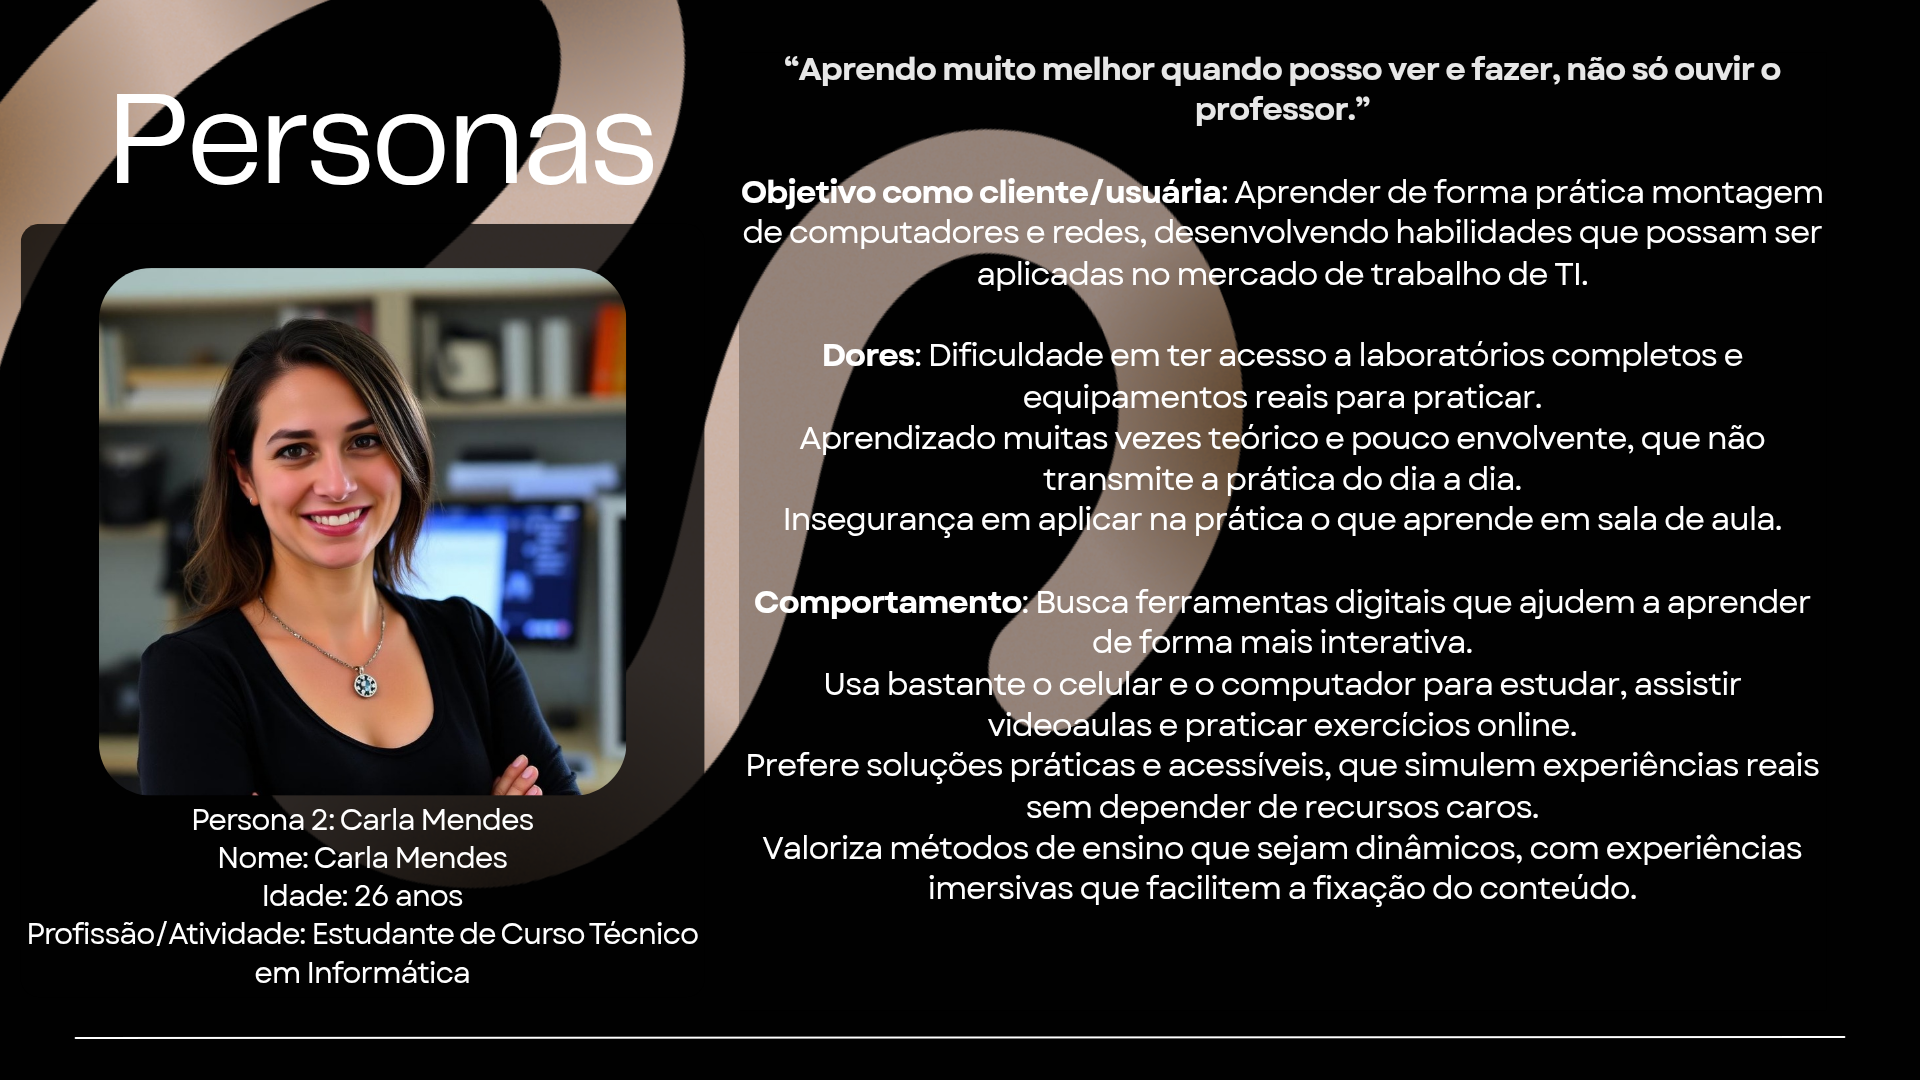
\includegraphics[width=\textwidth]{imgs/briefing_persona02.png}
    \caption{Persona 2: Carla Mendes.}
    \label{fig:persona02}
\end{subfigure}
\caption{Personas consideradas no projeto SAVIT.}
\end{figure}

\section{Website: Estrutura e Especificações Técnicas}
O website da equipe Orbi apresenta o projeto, integra a criação de contas e disponibiliza o download do APK para Android.

\subsection{Mapa do site}
O mapa do site representa a organização e a navegação entre as páginas do website.

\begin{figure}[H]
\centering
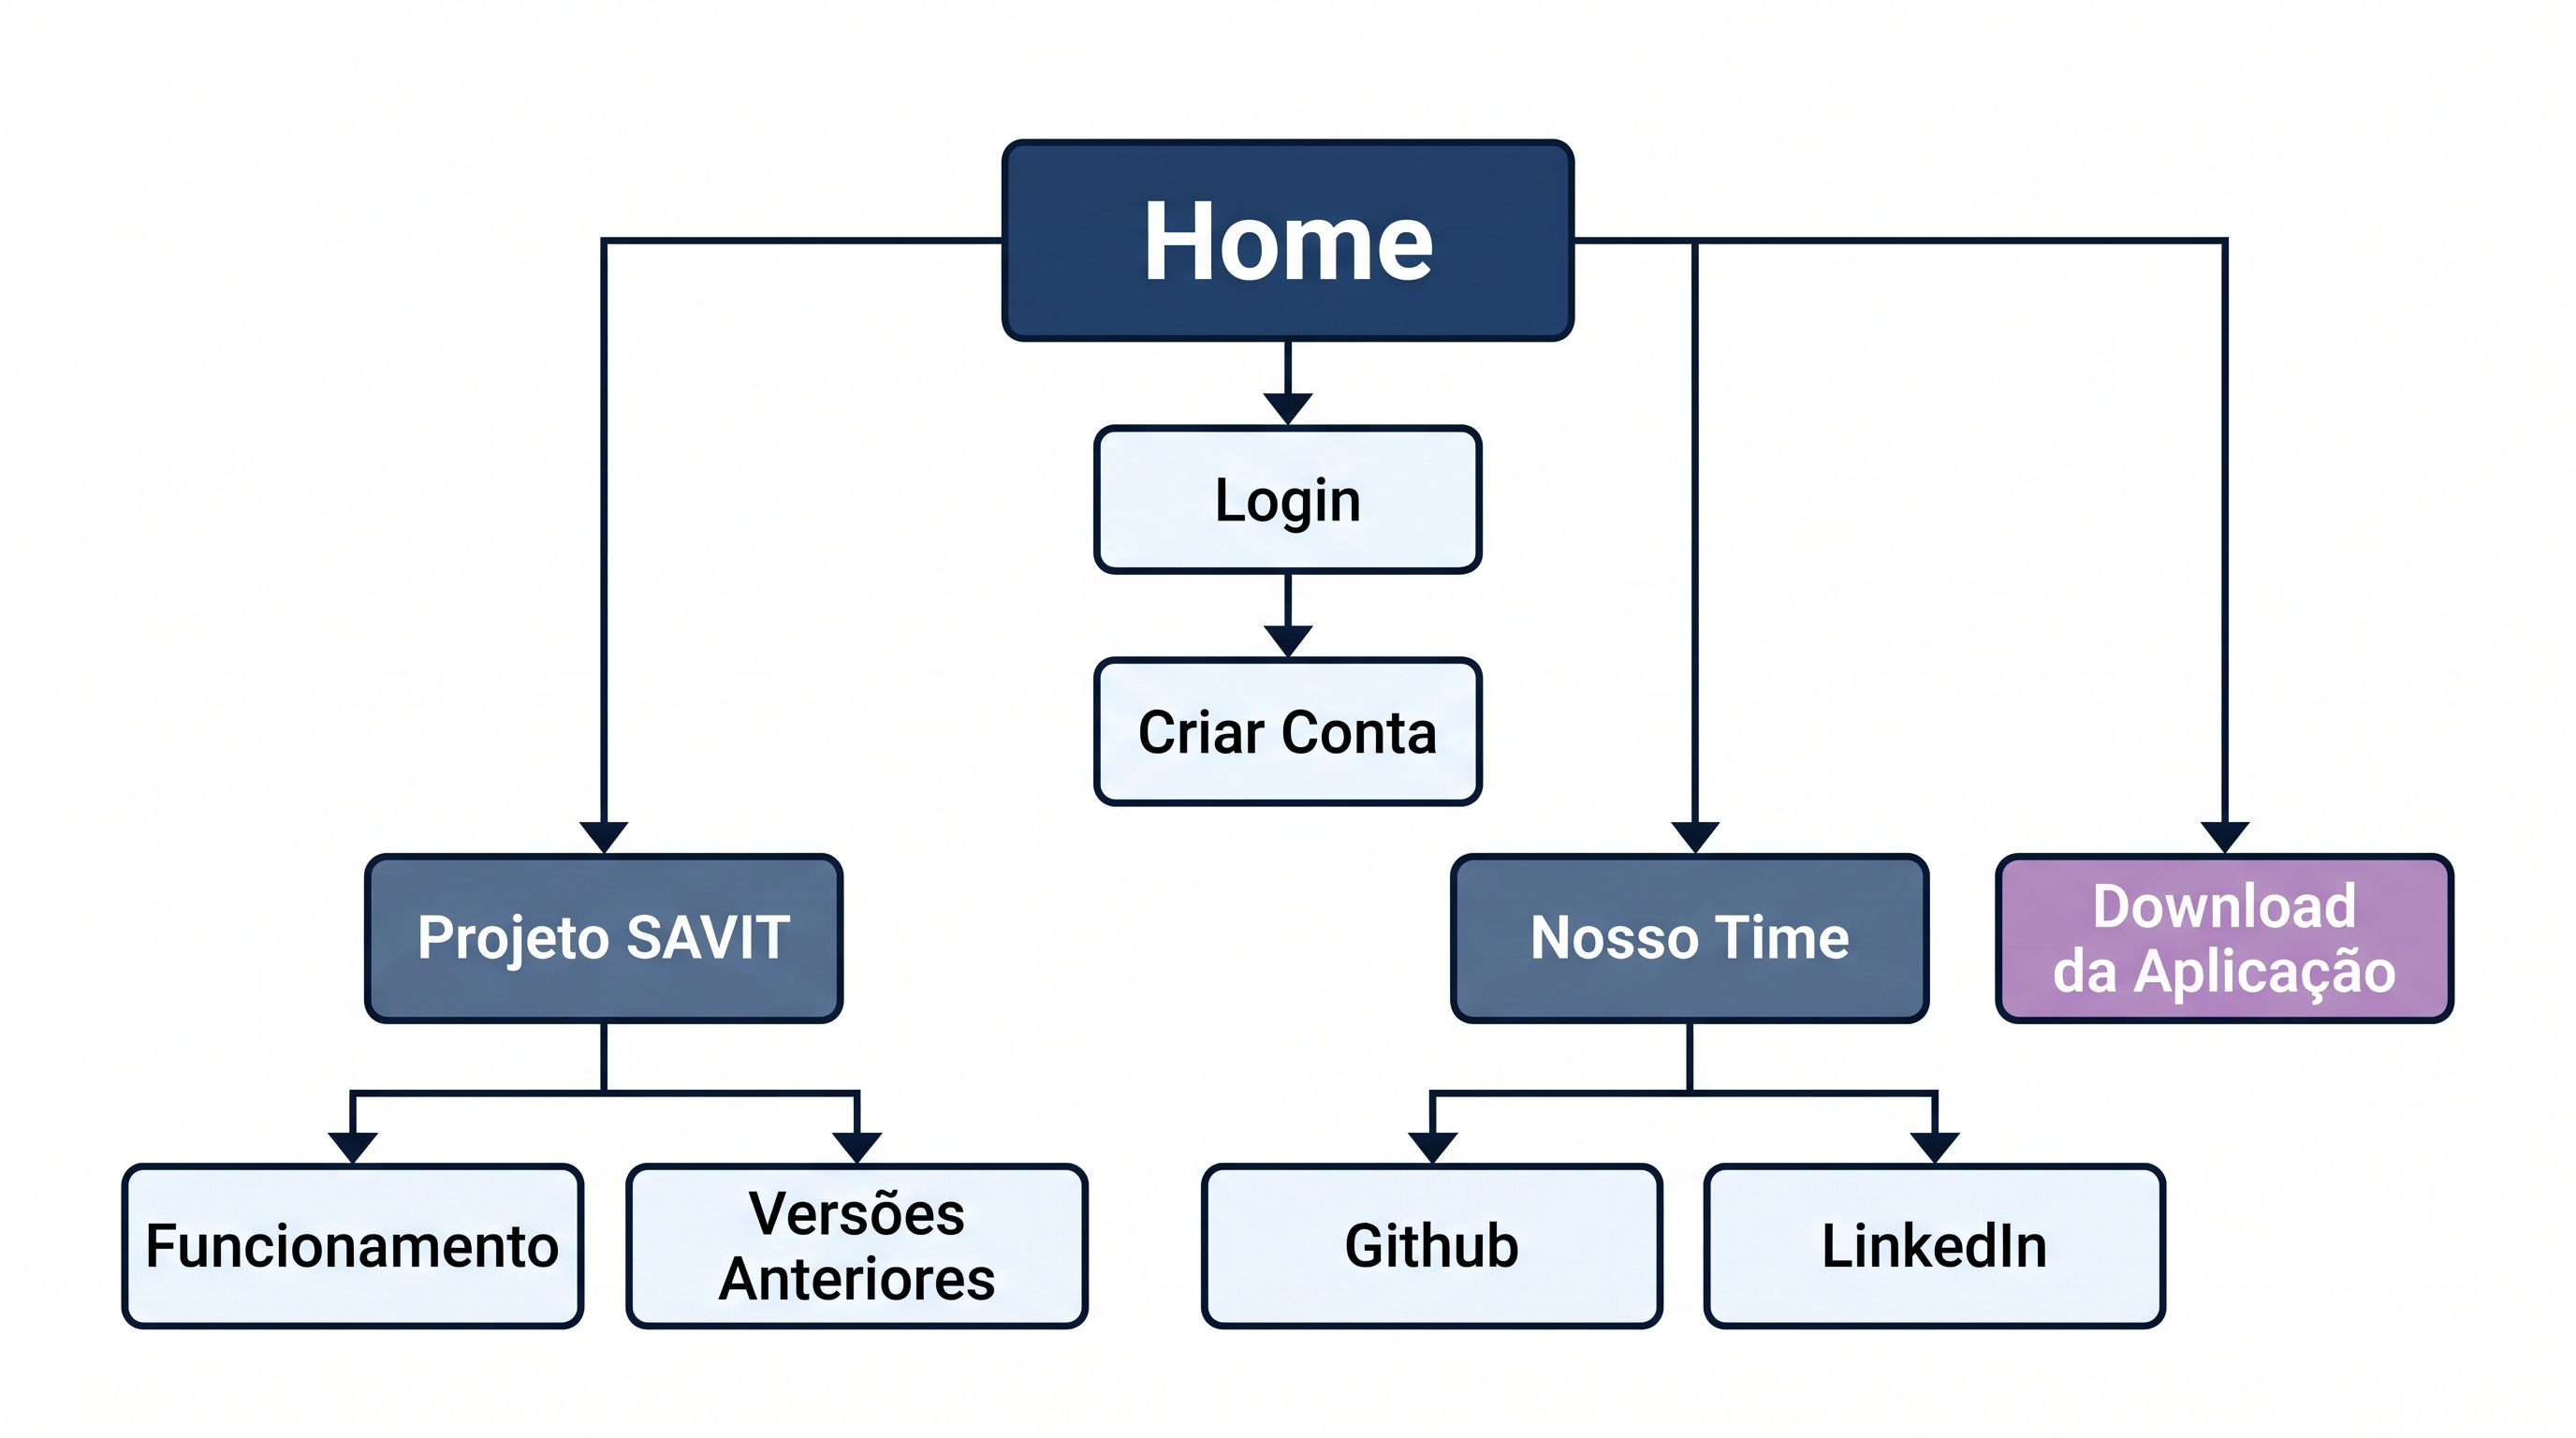
\includegraphics[width=0.9\textwidth]{imgs/website-mapa.png}
\caption{Estrutura de navegação do website da equipe.}
\label{fig:sitemap}
\end{figure}

\subsection{Páginas do website}
As páginas a seguir exibem a estrutura Web final para suporte ao projeto.

\begin{figure}[H]
\centering
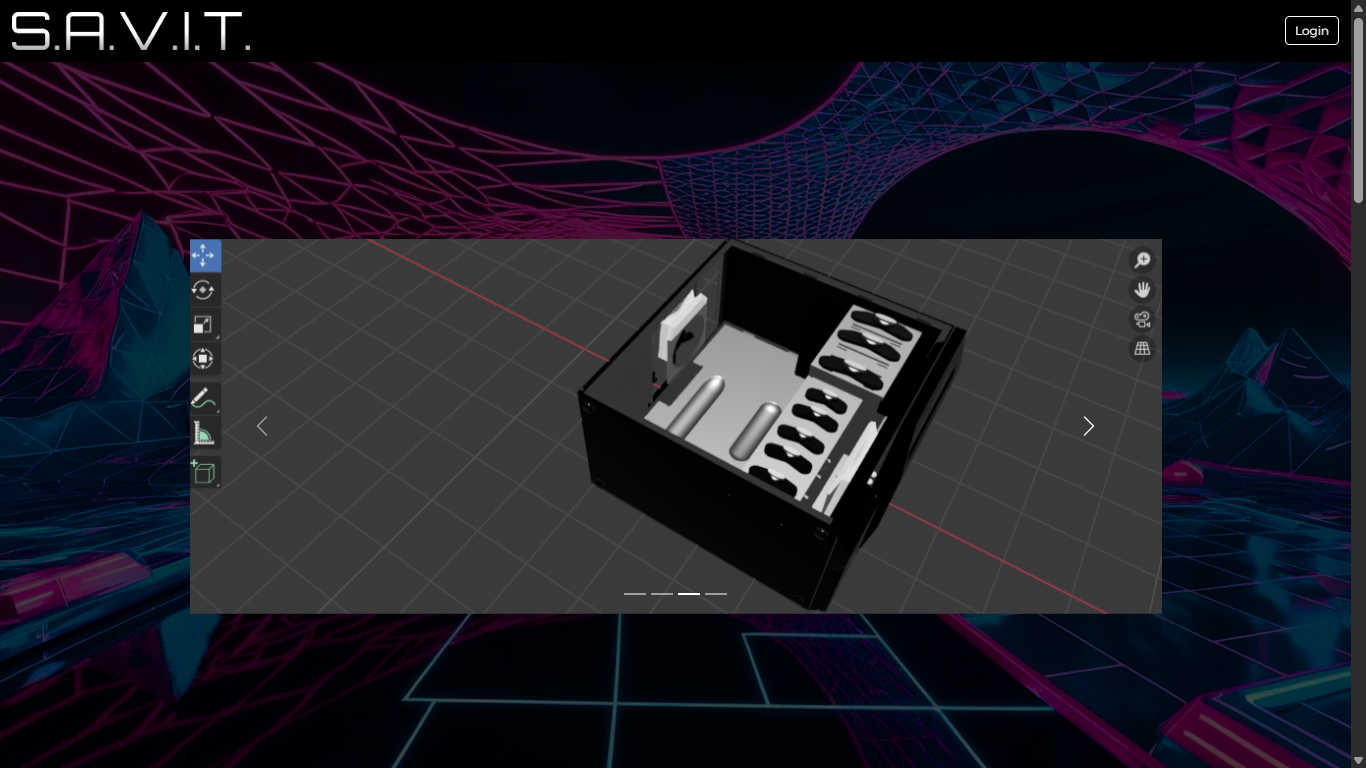
\includegraphics[width=0.8\textwidth]{imgs/website-home.png}
\caption{Página inicial do website da equipe.}
\label{fig:website-home}
\end{figure}

\begin{figure}[H]
\centering
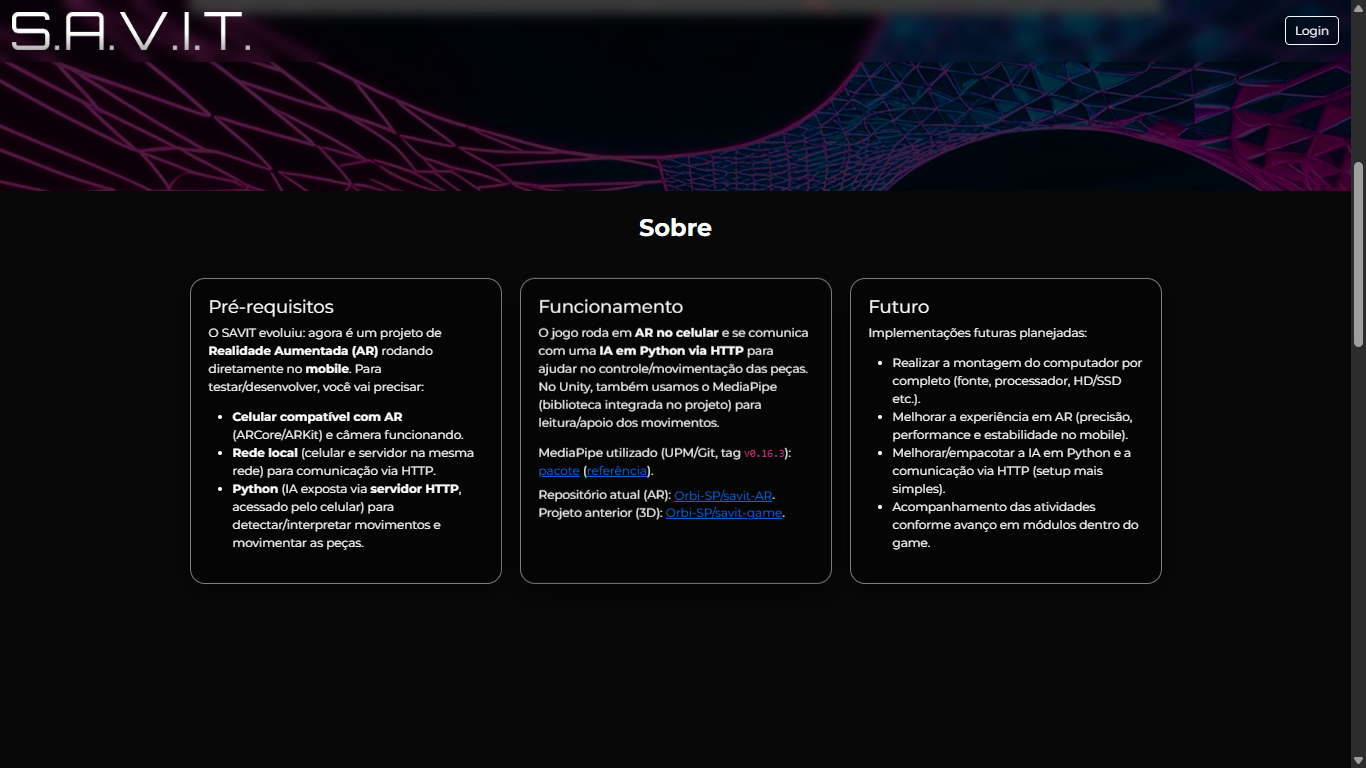
\includegraphics[width=0.8\textwidth]{imgs/website-projeto.png}
\caption{Página de apresentação do projeto SAVIT.}
\label{fig:website-projeto}
\end{figure}

\begin{figure}[H]
\centering
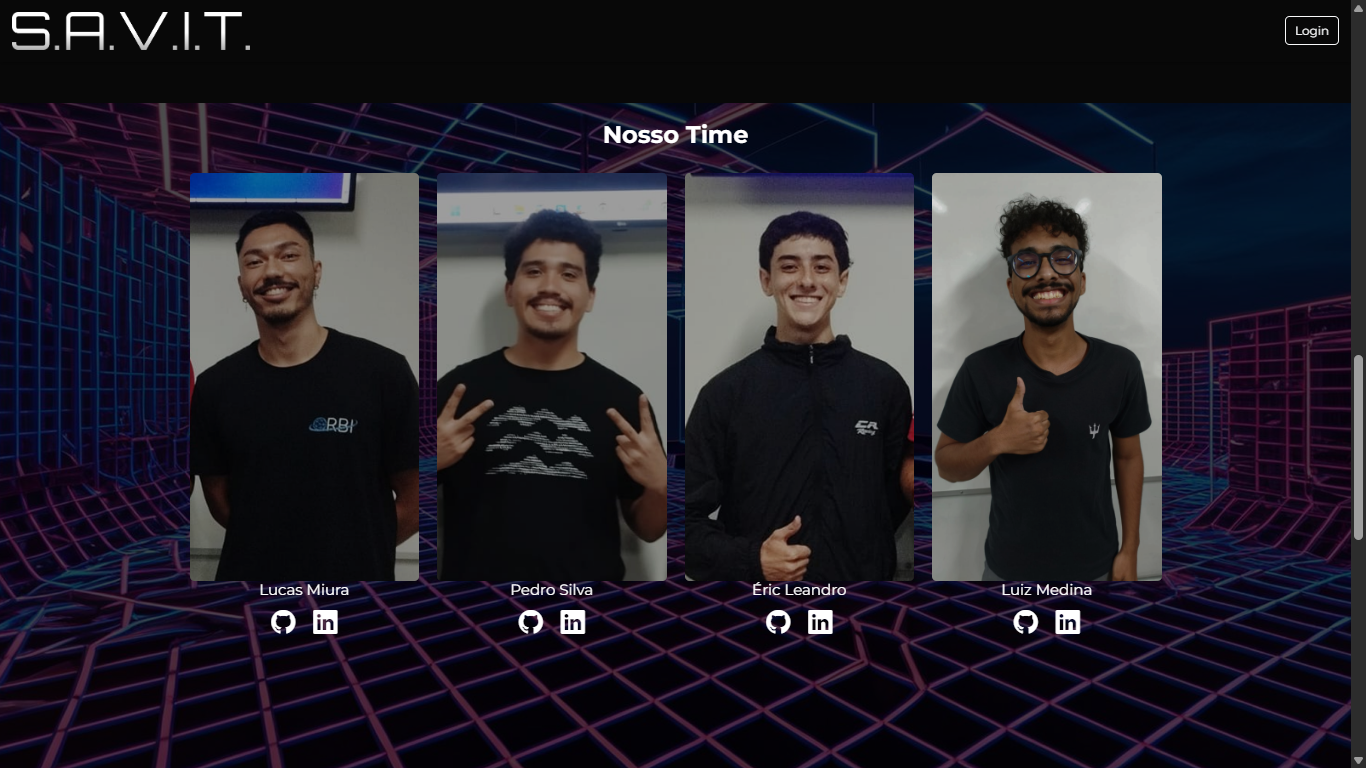
\includegraphics[width=0.8\textwidth]{imgs/website-equipe.png}
\caption{Página de apresentação da equipe Orbi.}
\label{fig:website-equipe}
\end{figure}

\begin{figure}[H]
\centering
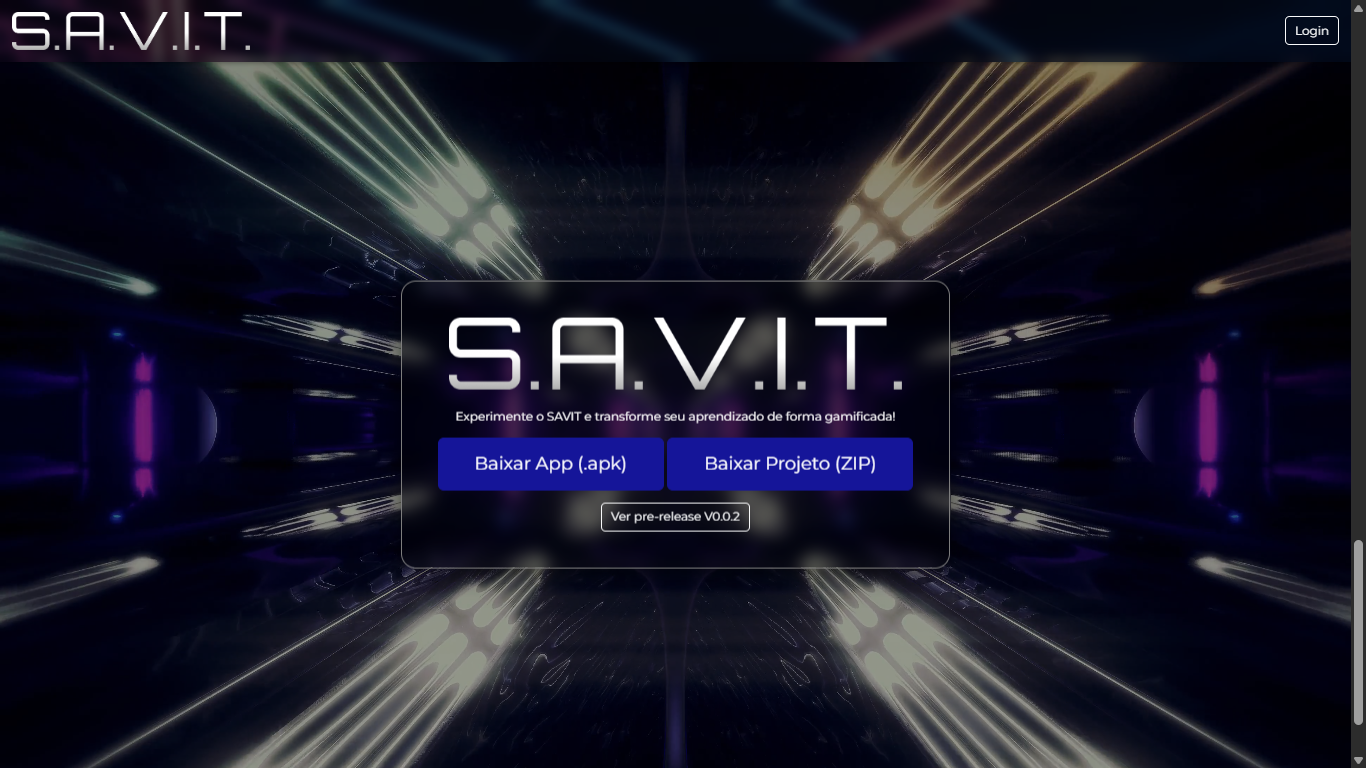
\includegraphics[width=0.8\textwidth]{imgs/website-download.png}
\caption{Página de download da aplicação.}
\label{fig:website-download}
\end{figure}

\begin{figure}[H]
\centering
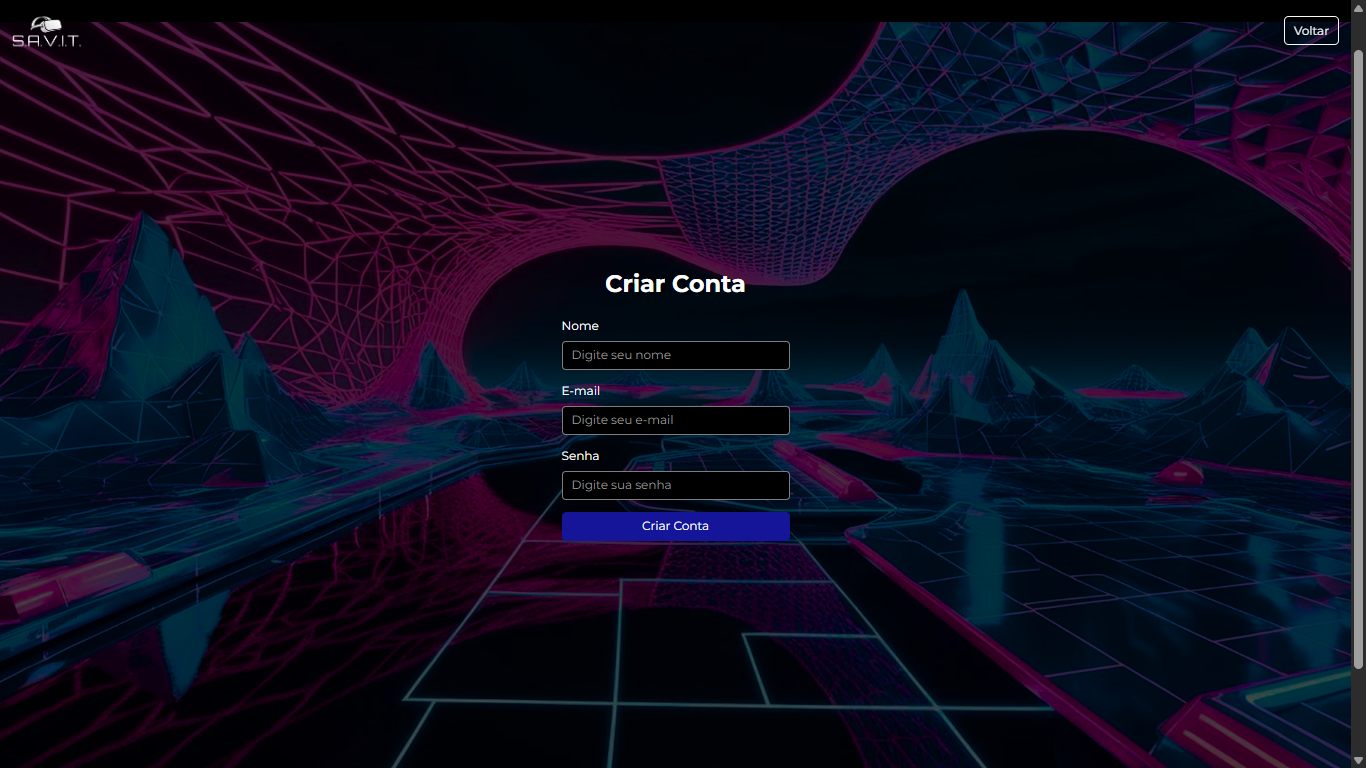
\includegraphics[width=0.8\textwidth]{imgs/website-conta.png}
\caption{Página de criação de conta no website.}
\label{fig:website-conta}
\end{figure}

\section{Capturas da Aplicação Móvel (Android / Realidade Aumentada)}
A aplicação móvel desenvolvida na Unity 6000 integra autenticação, rastreamento de gestos com MediaPipe, detecção de superfícies em AR, instrução tutorial e ranking global.

\subsection{Autenticação e Menu Principal}
\begin{figure}[H]
\centering
\begin{subfigure}[t]{0.45\textwidth}
    \centering
    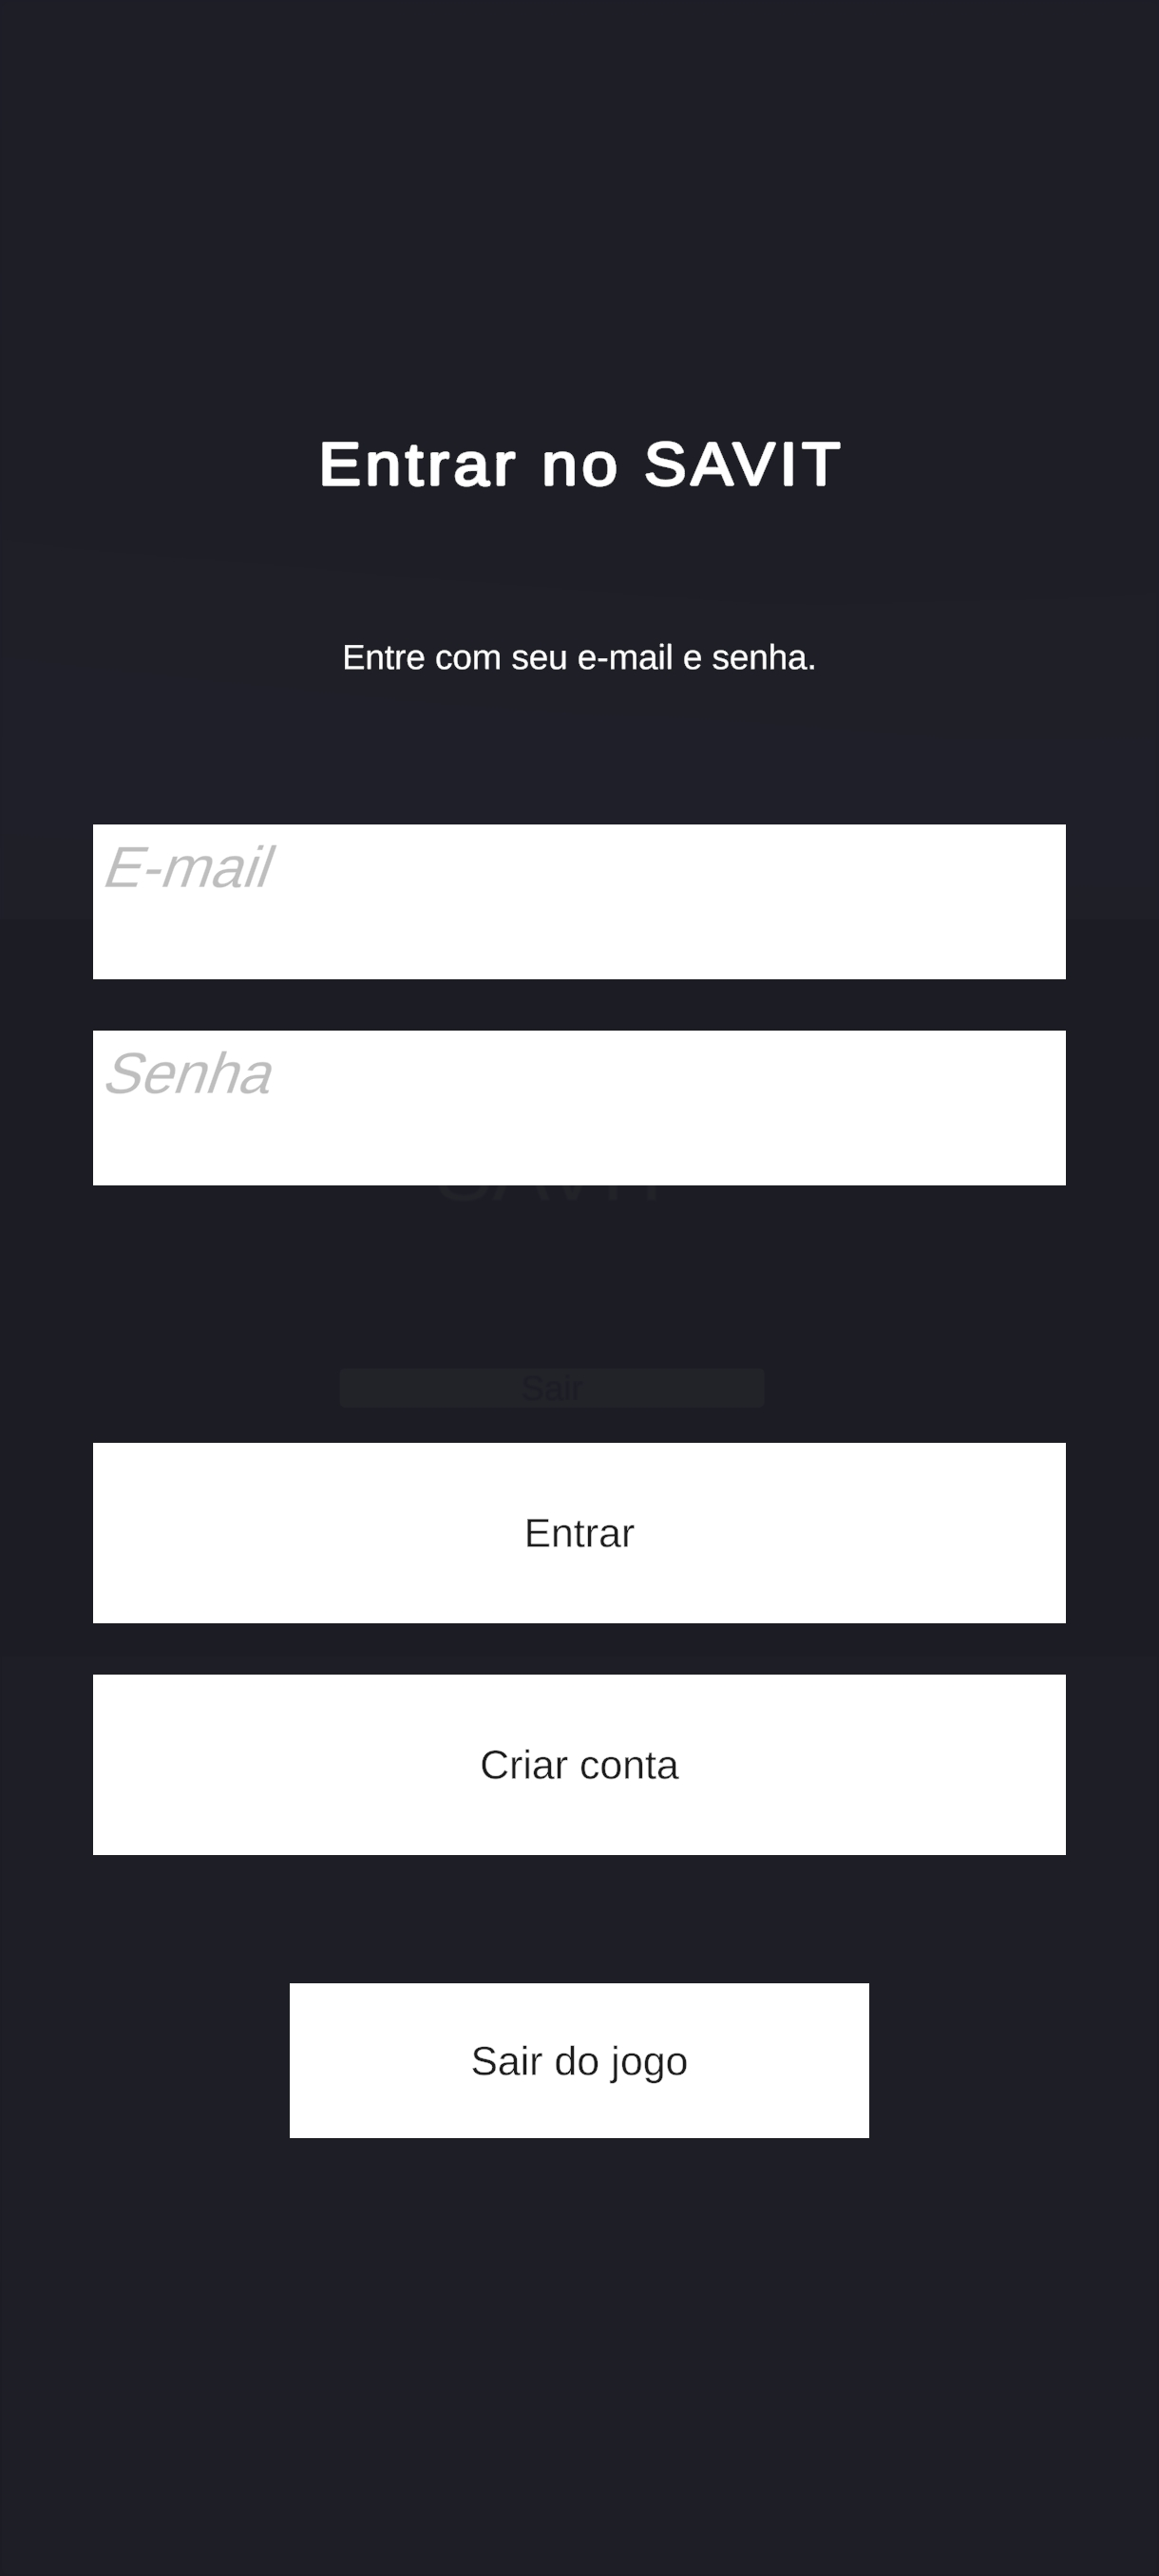
\includegraphics[width=\textwidth]{imgs/savit-login.png}
    \caption{Tela de Autenticação / Login do aplicativo.}
    \label{fig:app-login}
\end{subfigure}
\hfill
\begin{subfigure}[t]{0.48\textwidth}
    \centering
    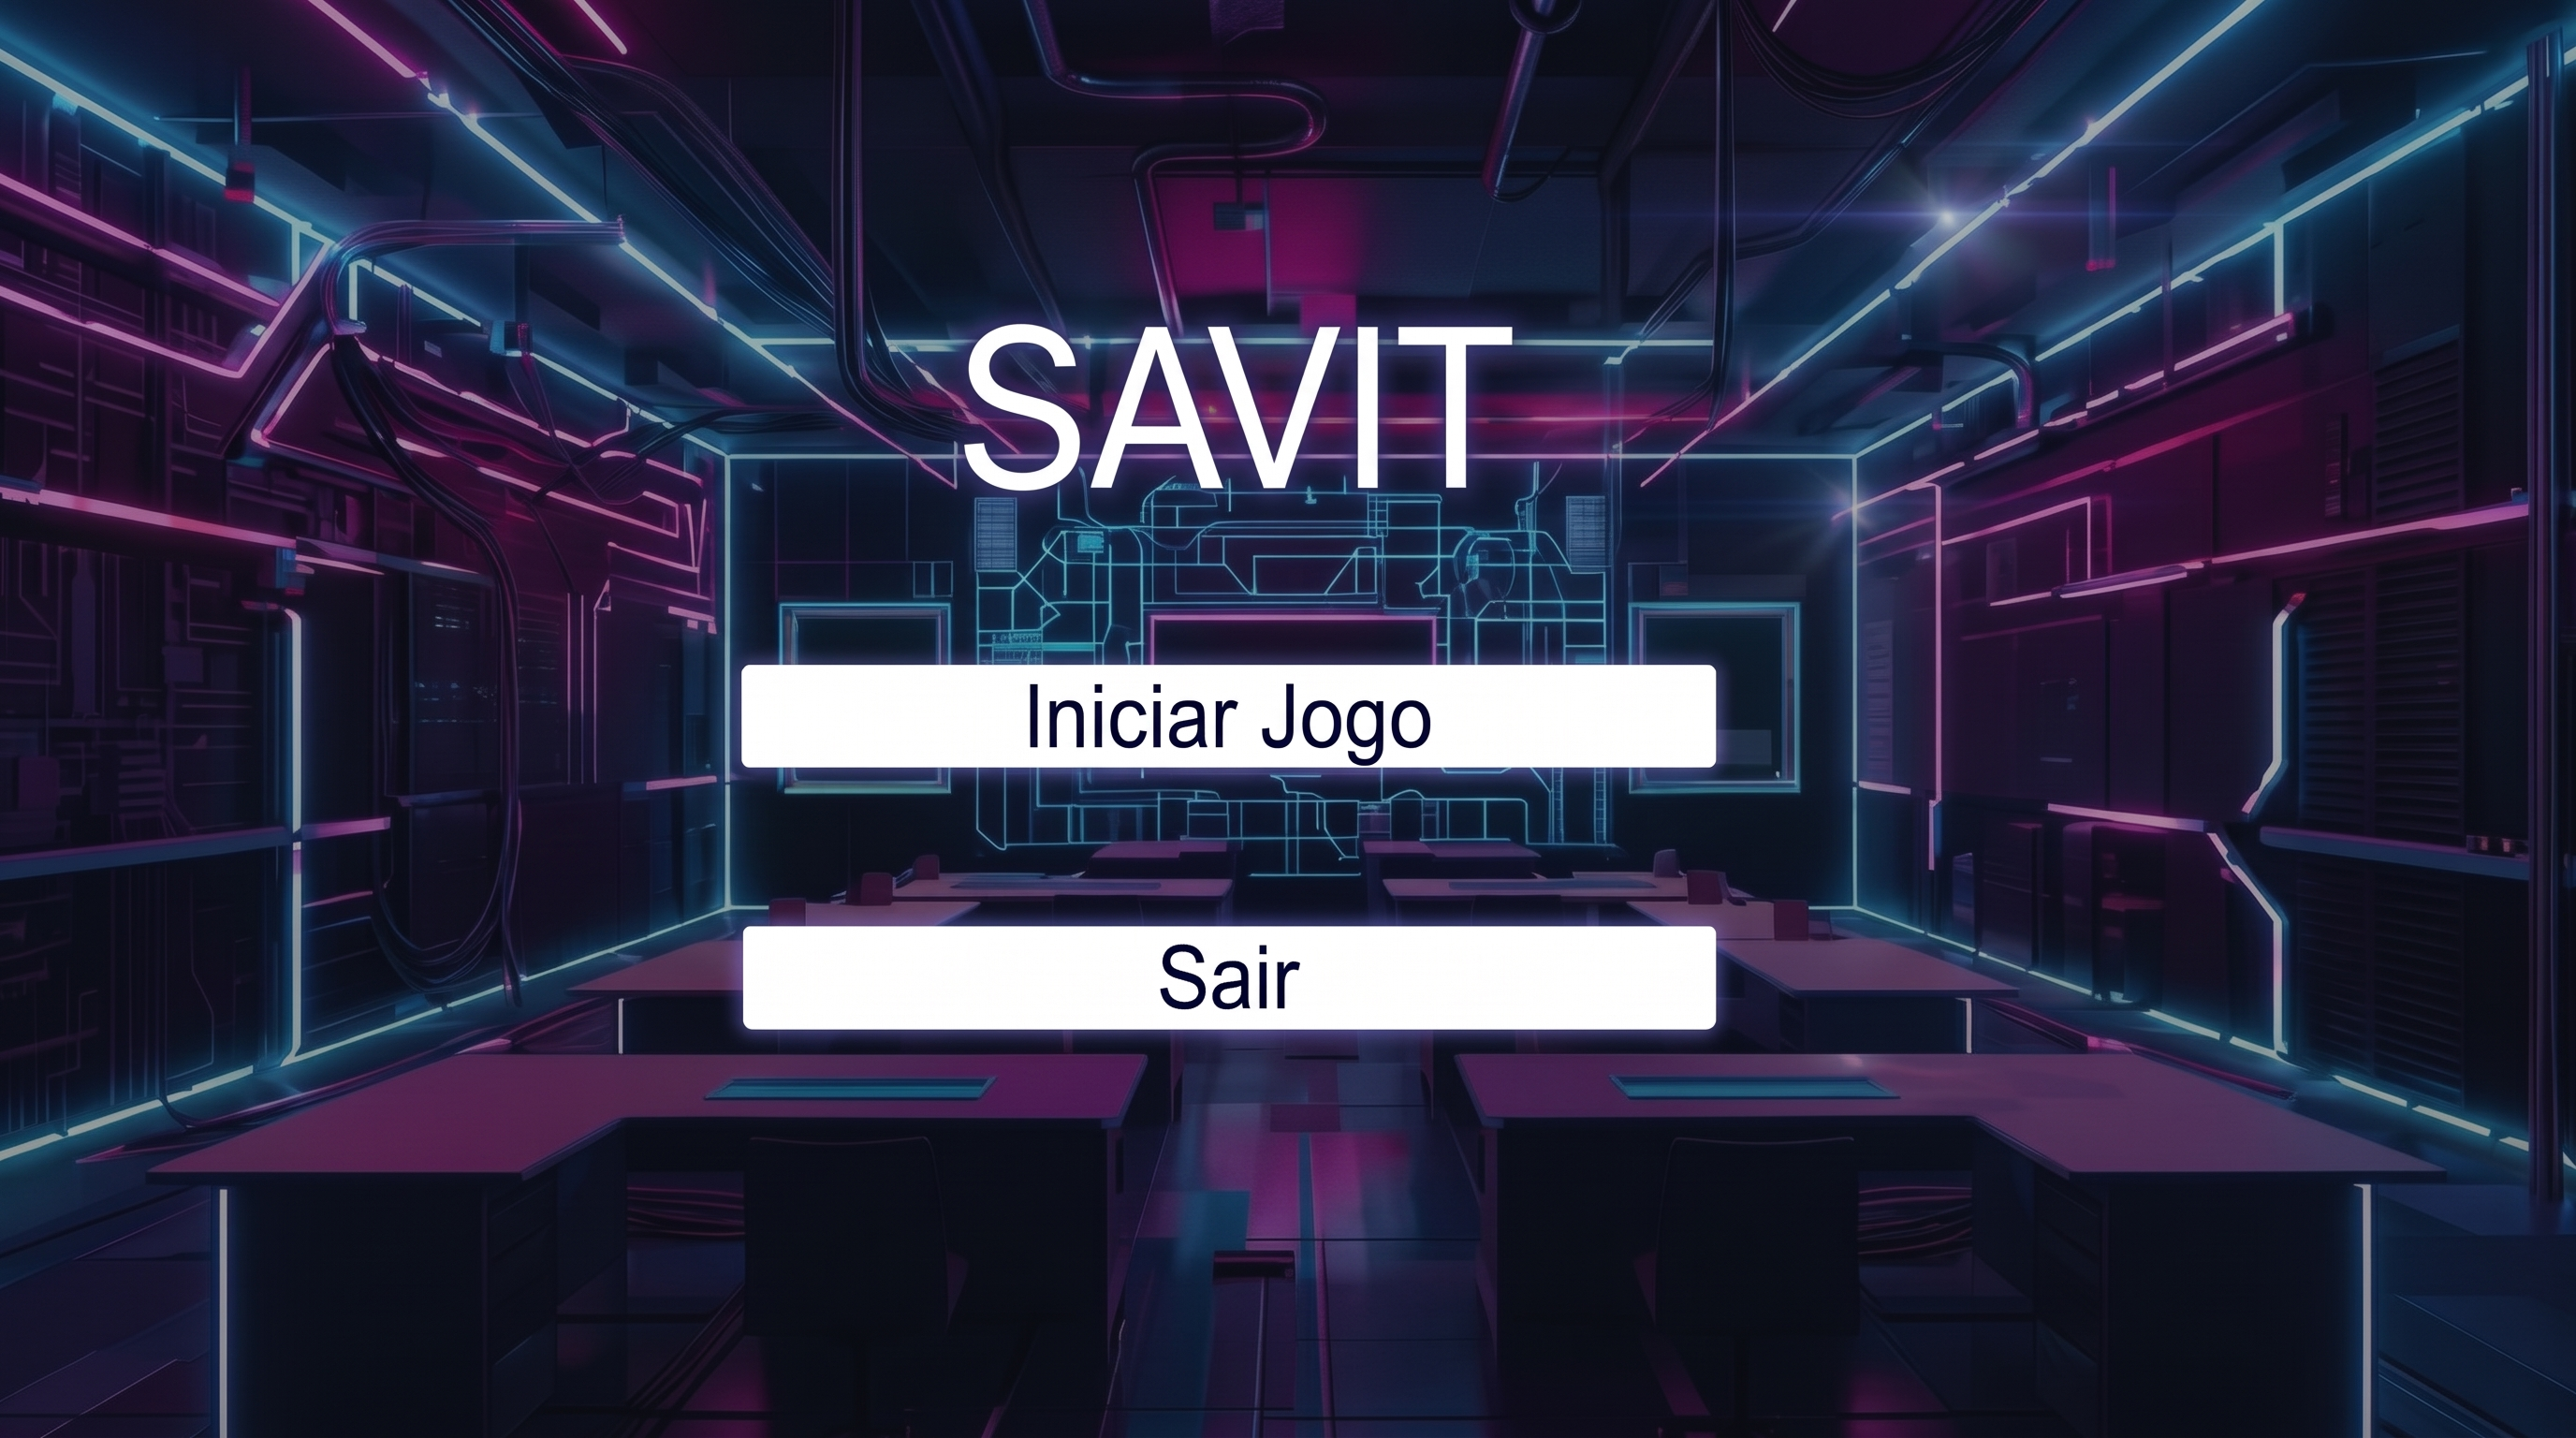
\includegraphics[width=\textwidth]{imgs/savit-menu-inicial.jpg}
    \caption{Menu Inicial da aplicação.}
    \label{fig:app-menu}
\end{subfigure}
\caption{Interfaces iniciais da aplicação móvel SAVIT.}
\end{figure}

\subsection{Posicionamento e Montagem em Realidade Aumentada}
\begin{figure}[H]
\centering
\begin{subfigure}[t]{0.48\textwidth}
    \centering
    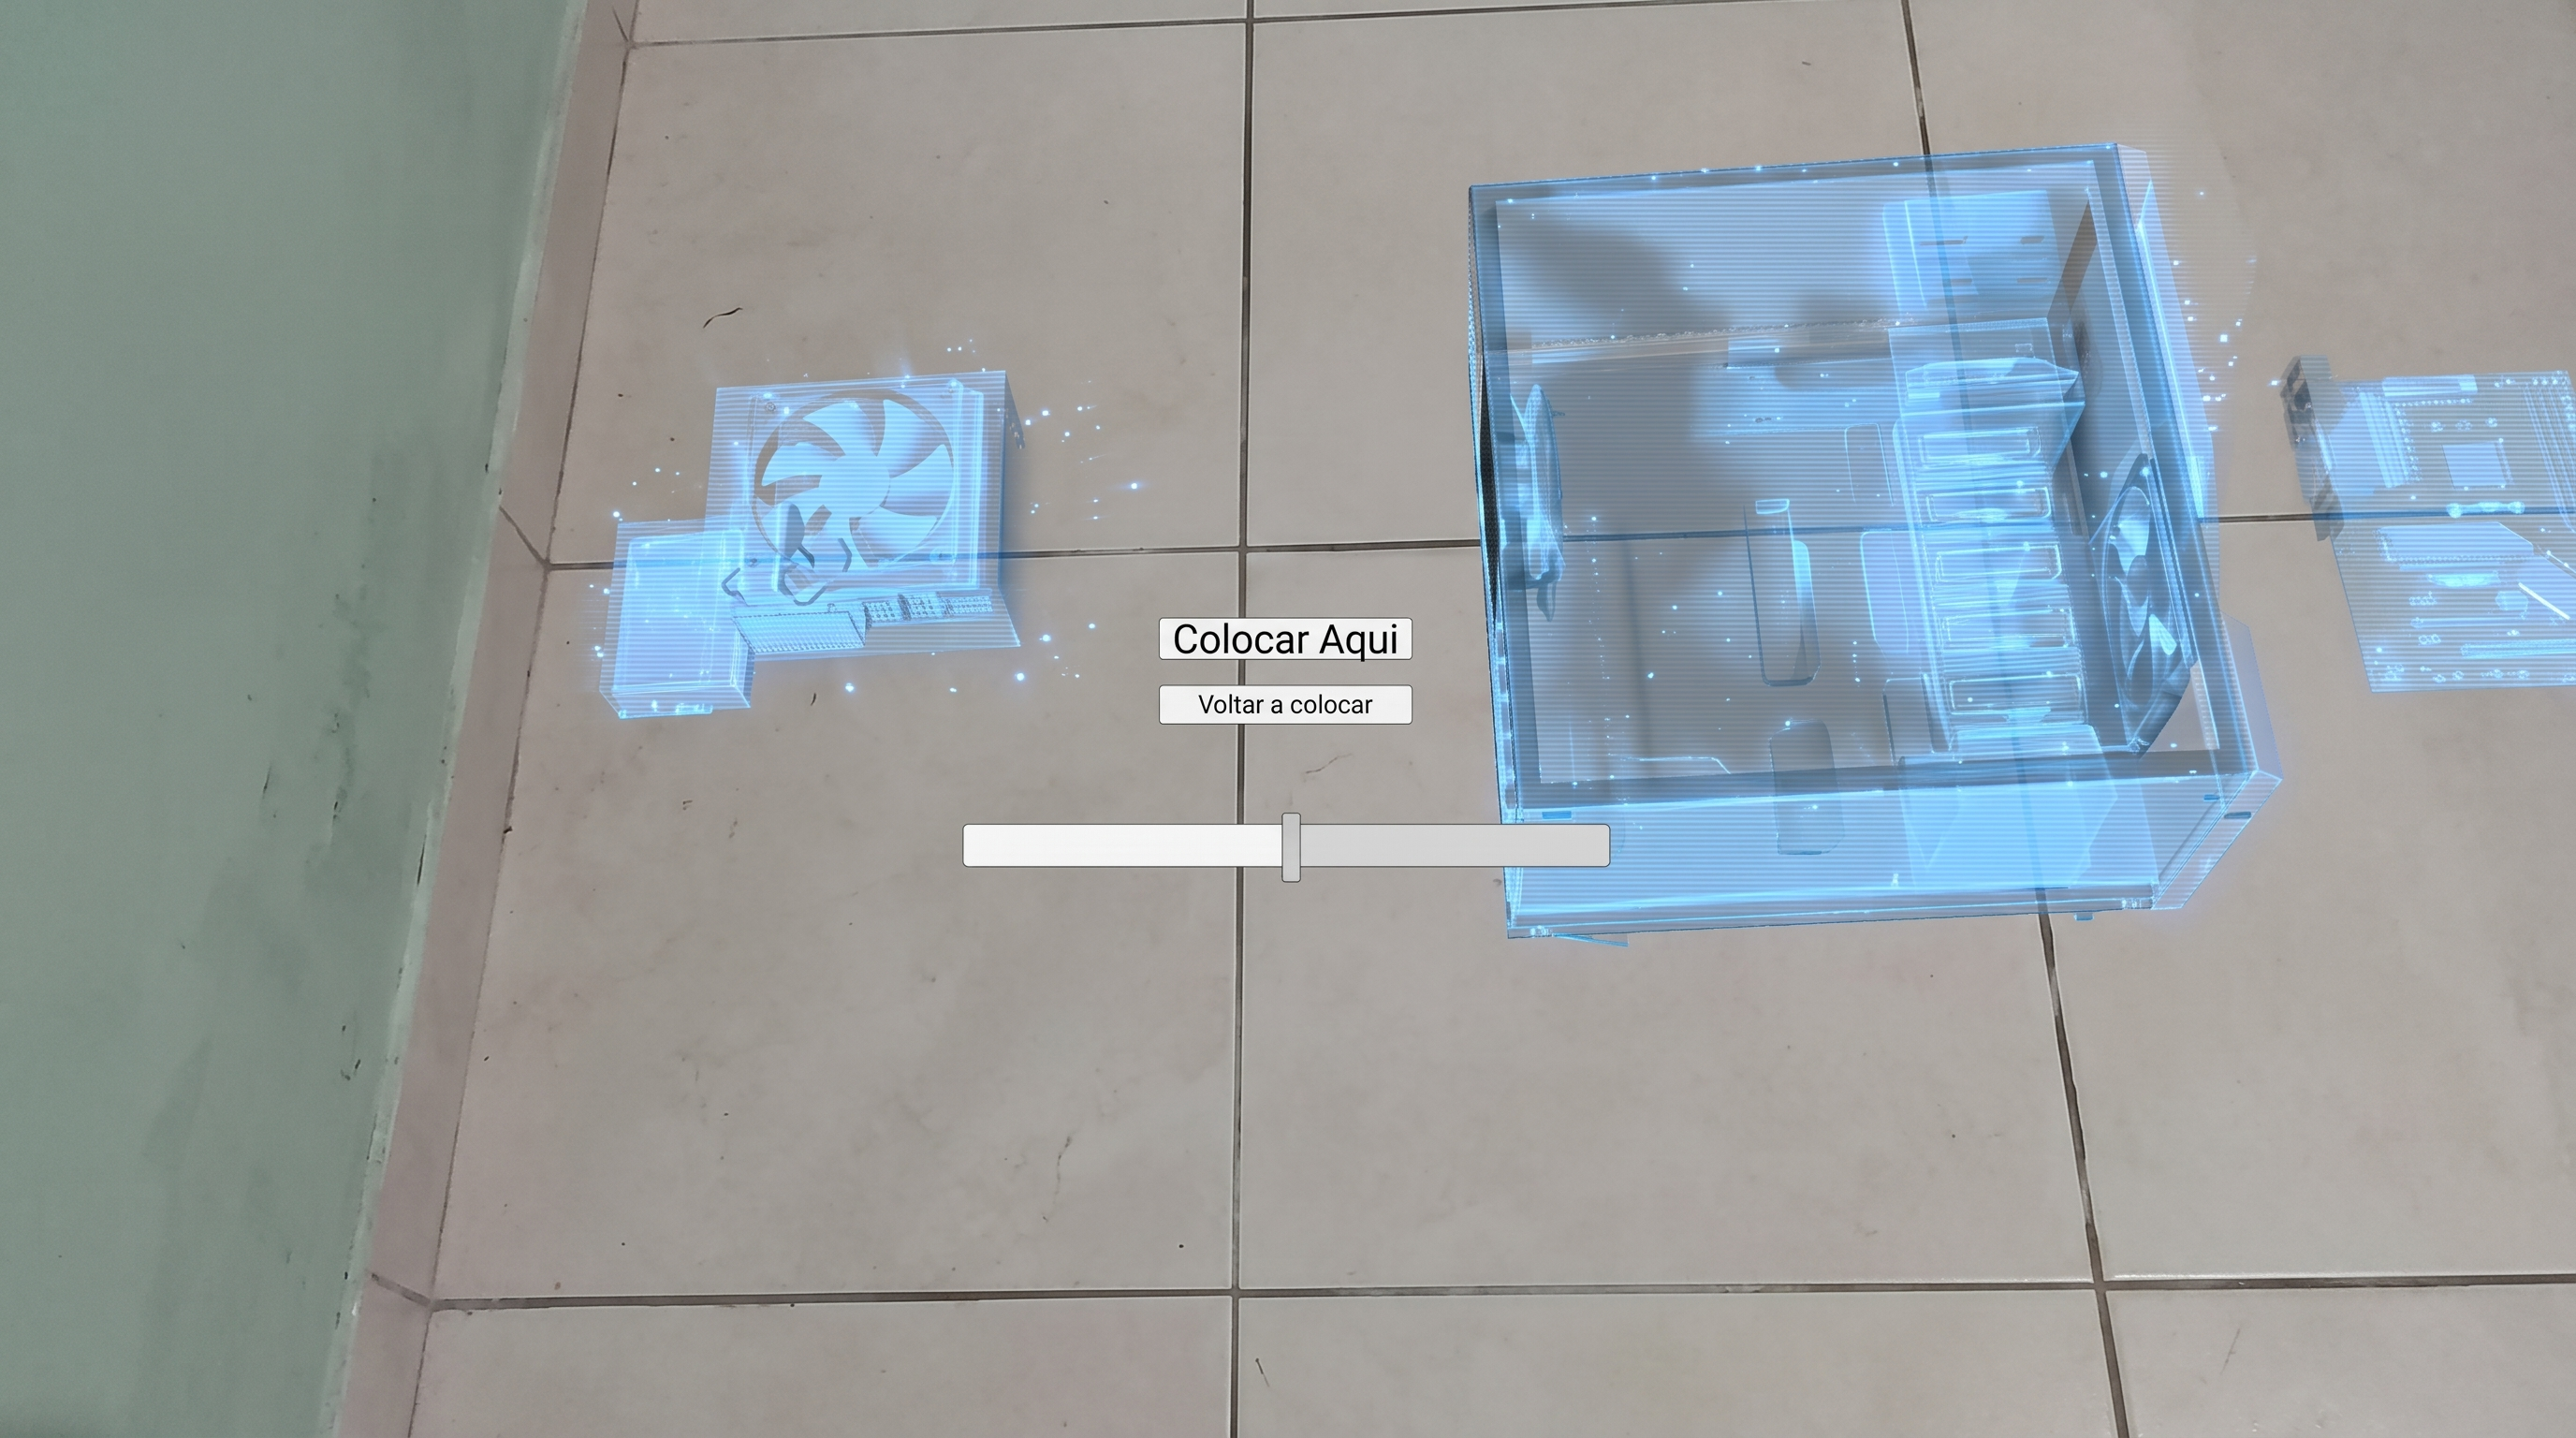
\includegraphics[width=\textwidth]{imgs/savit-posicionamento-pecas.jpg}
    \caption{Detecção de superfície e posicionamento em AR.}
    \label{fig:app-posicionamento}
\end{subfigure}
\hfill
\begin{subfigure}[t]{0.48\textwidth}
    \centering
    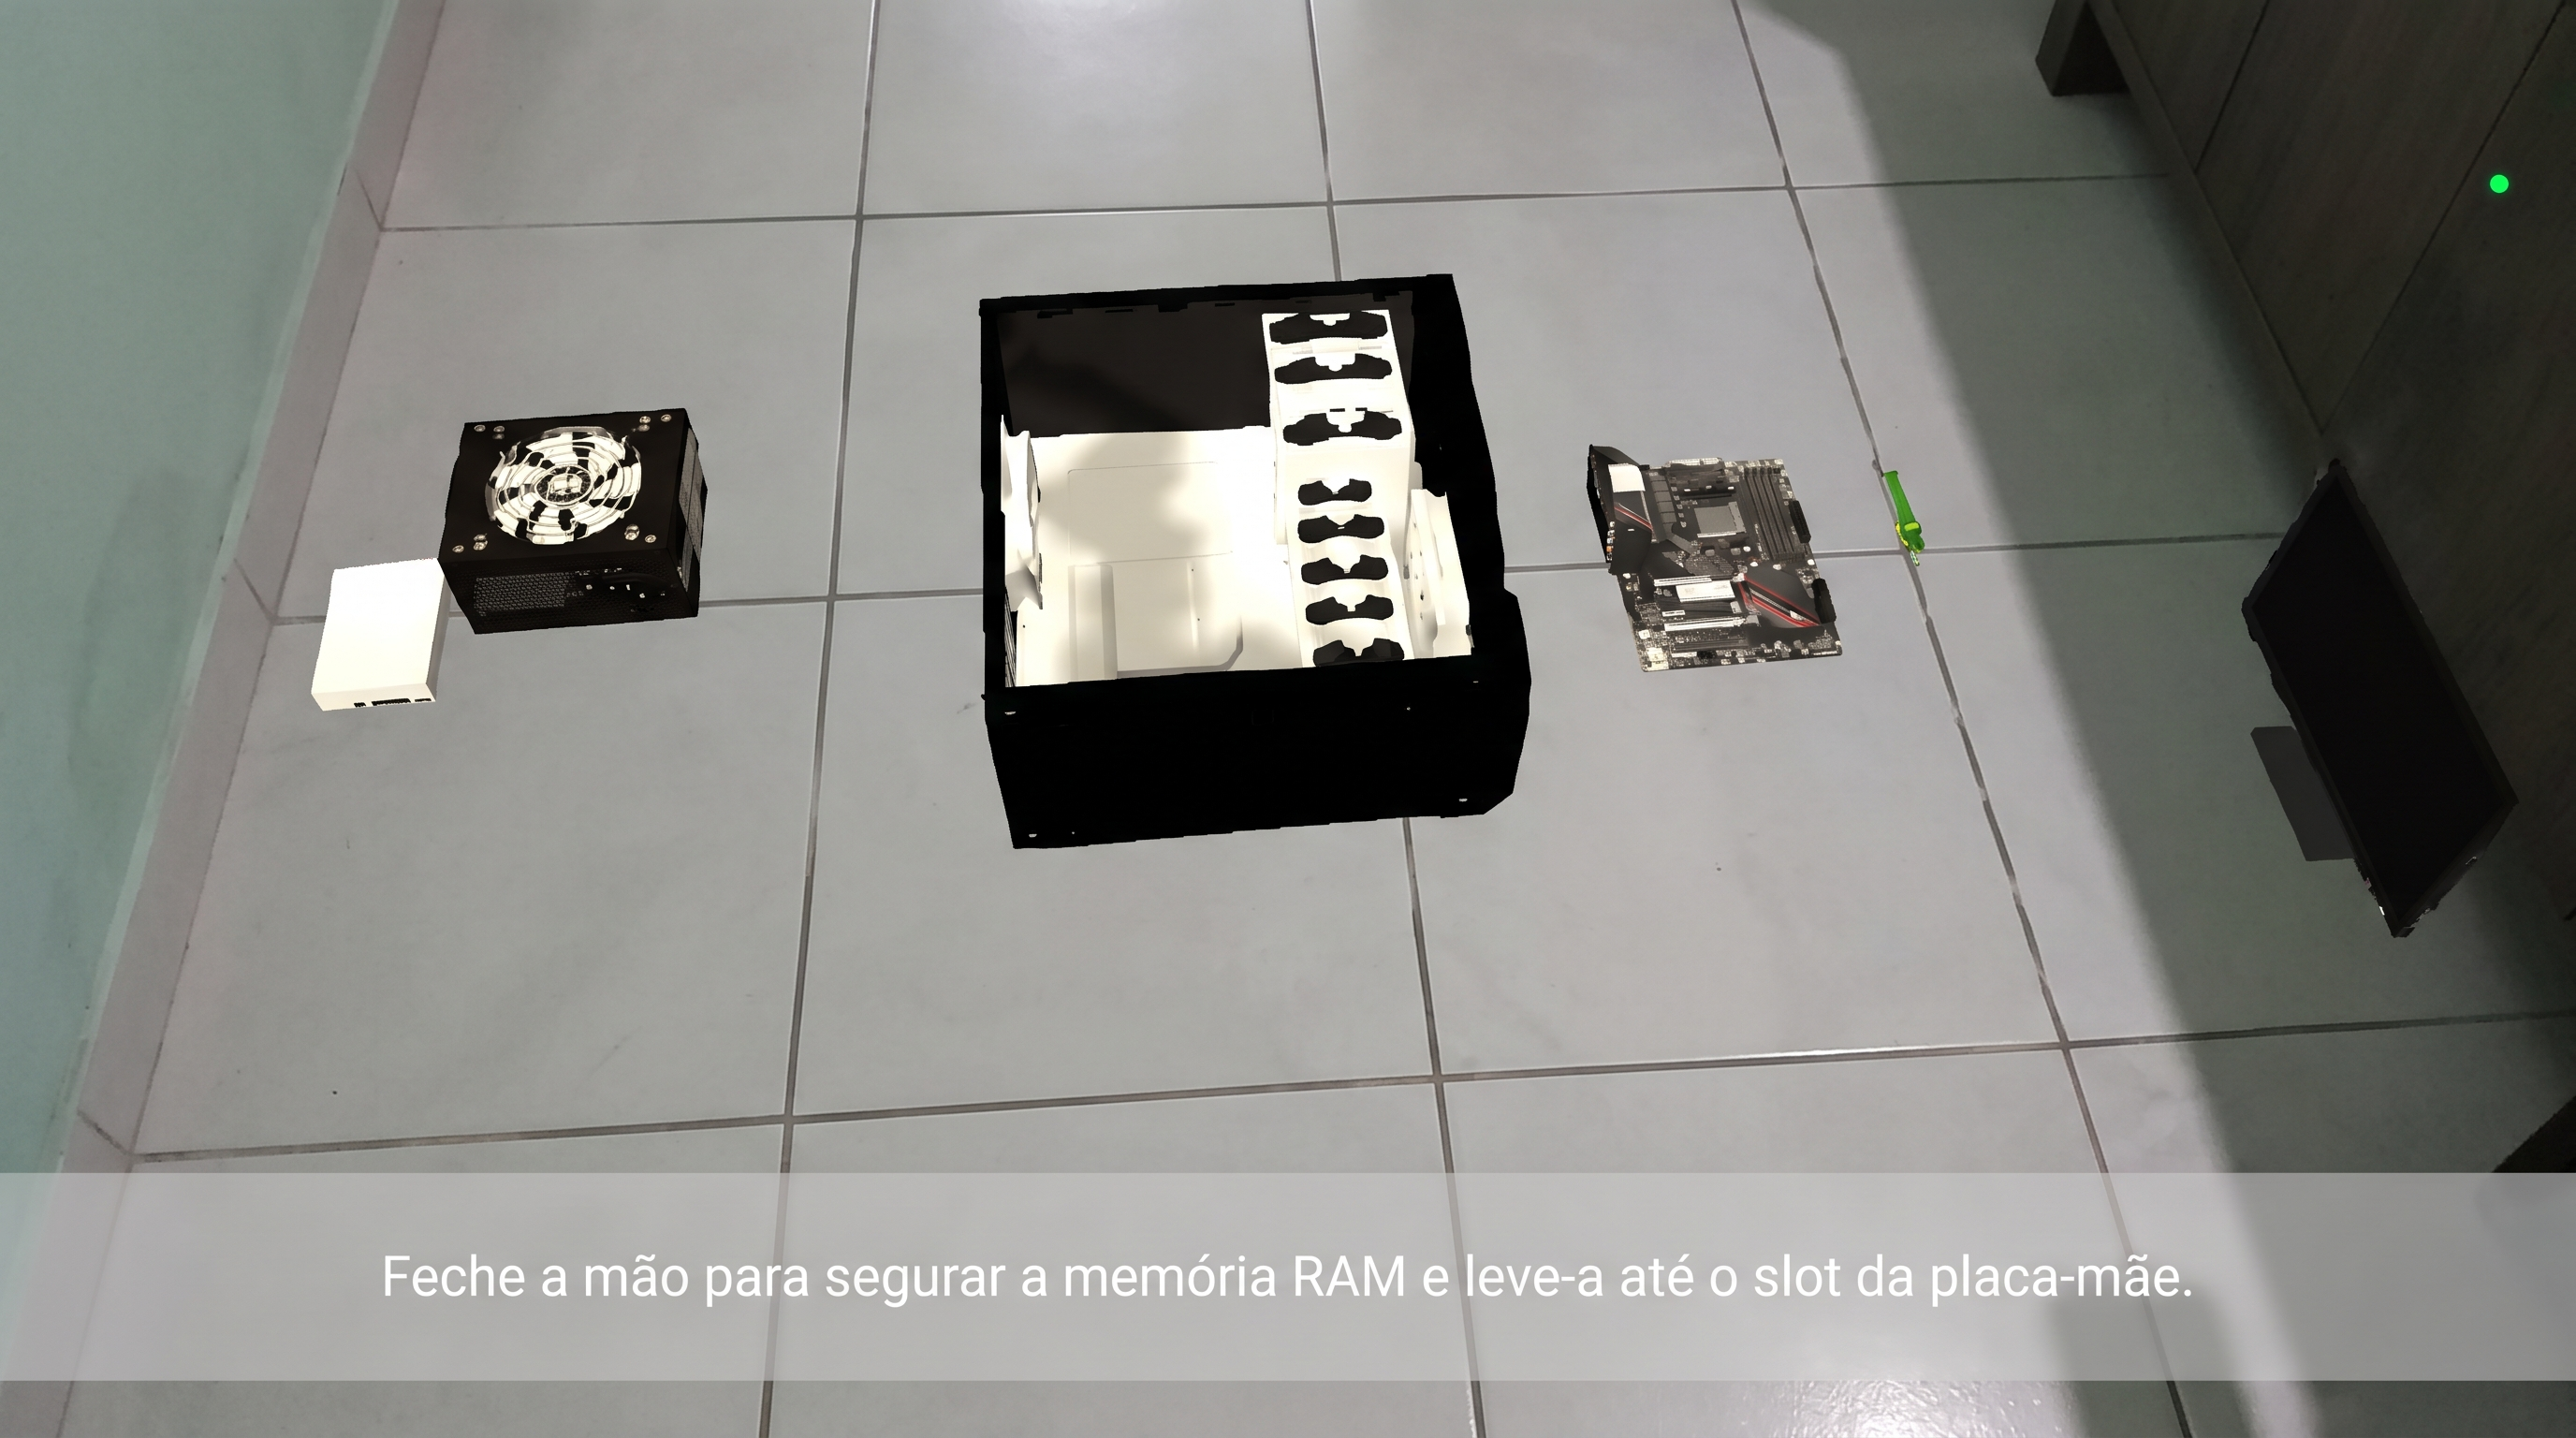
\includegraphics[width=\textwidth]{imgs/savit-modelagem-3d.jpg}
    \caption{Disposição dos componentes 3D no ambiente.}
    \label{fig:app-modelagem}
\end{subfigure}
\caption{Etapa de posicionamento dos modelos 3D no ambiente real.}
\end{figure}

\subsection{Interação por Gestos, Validação e Ranking}
\begin{figure}[H]
\centering
\begin{subfigure}[t]{0.48\textwidth}
    \centering
    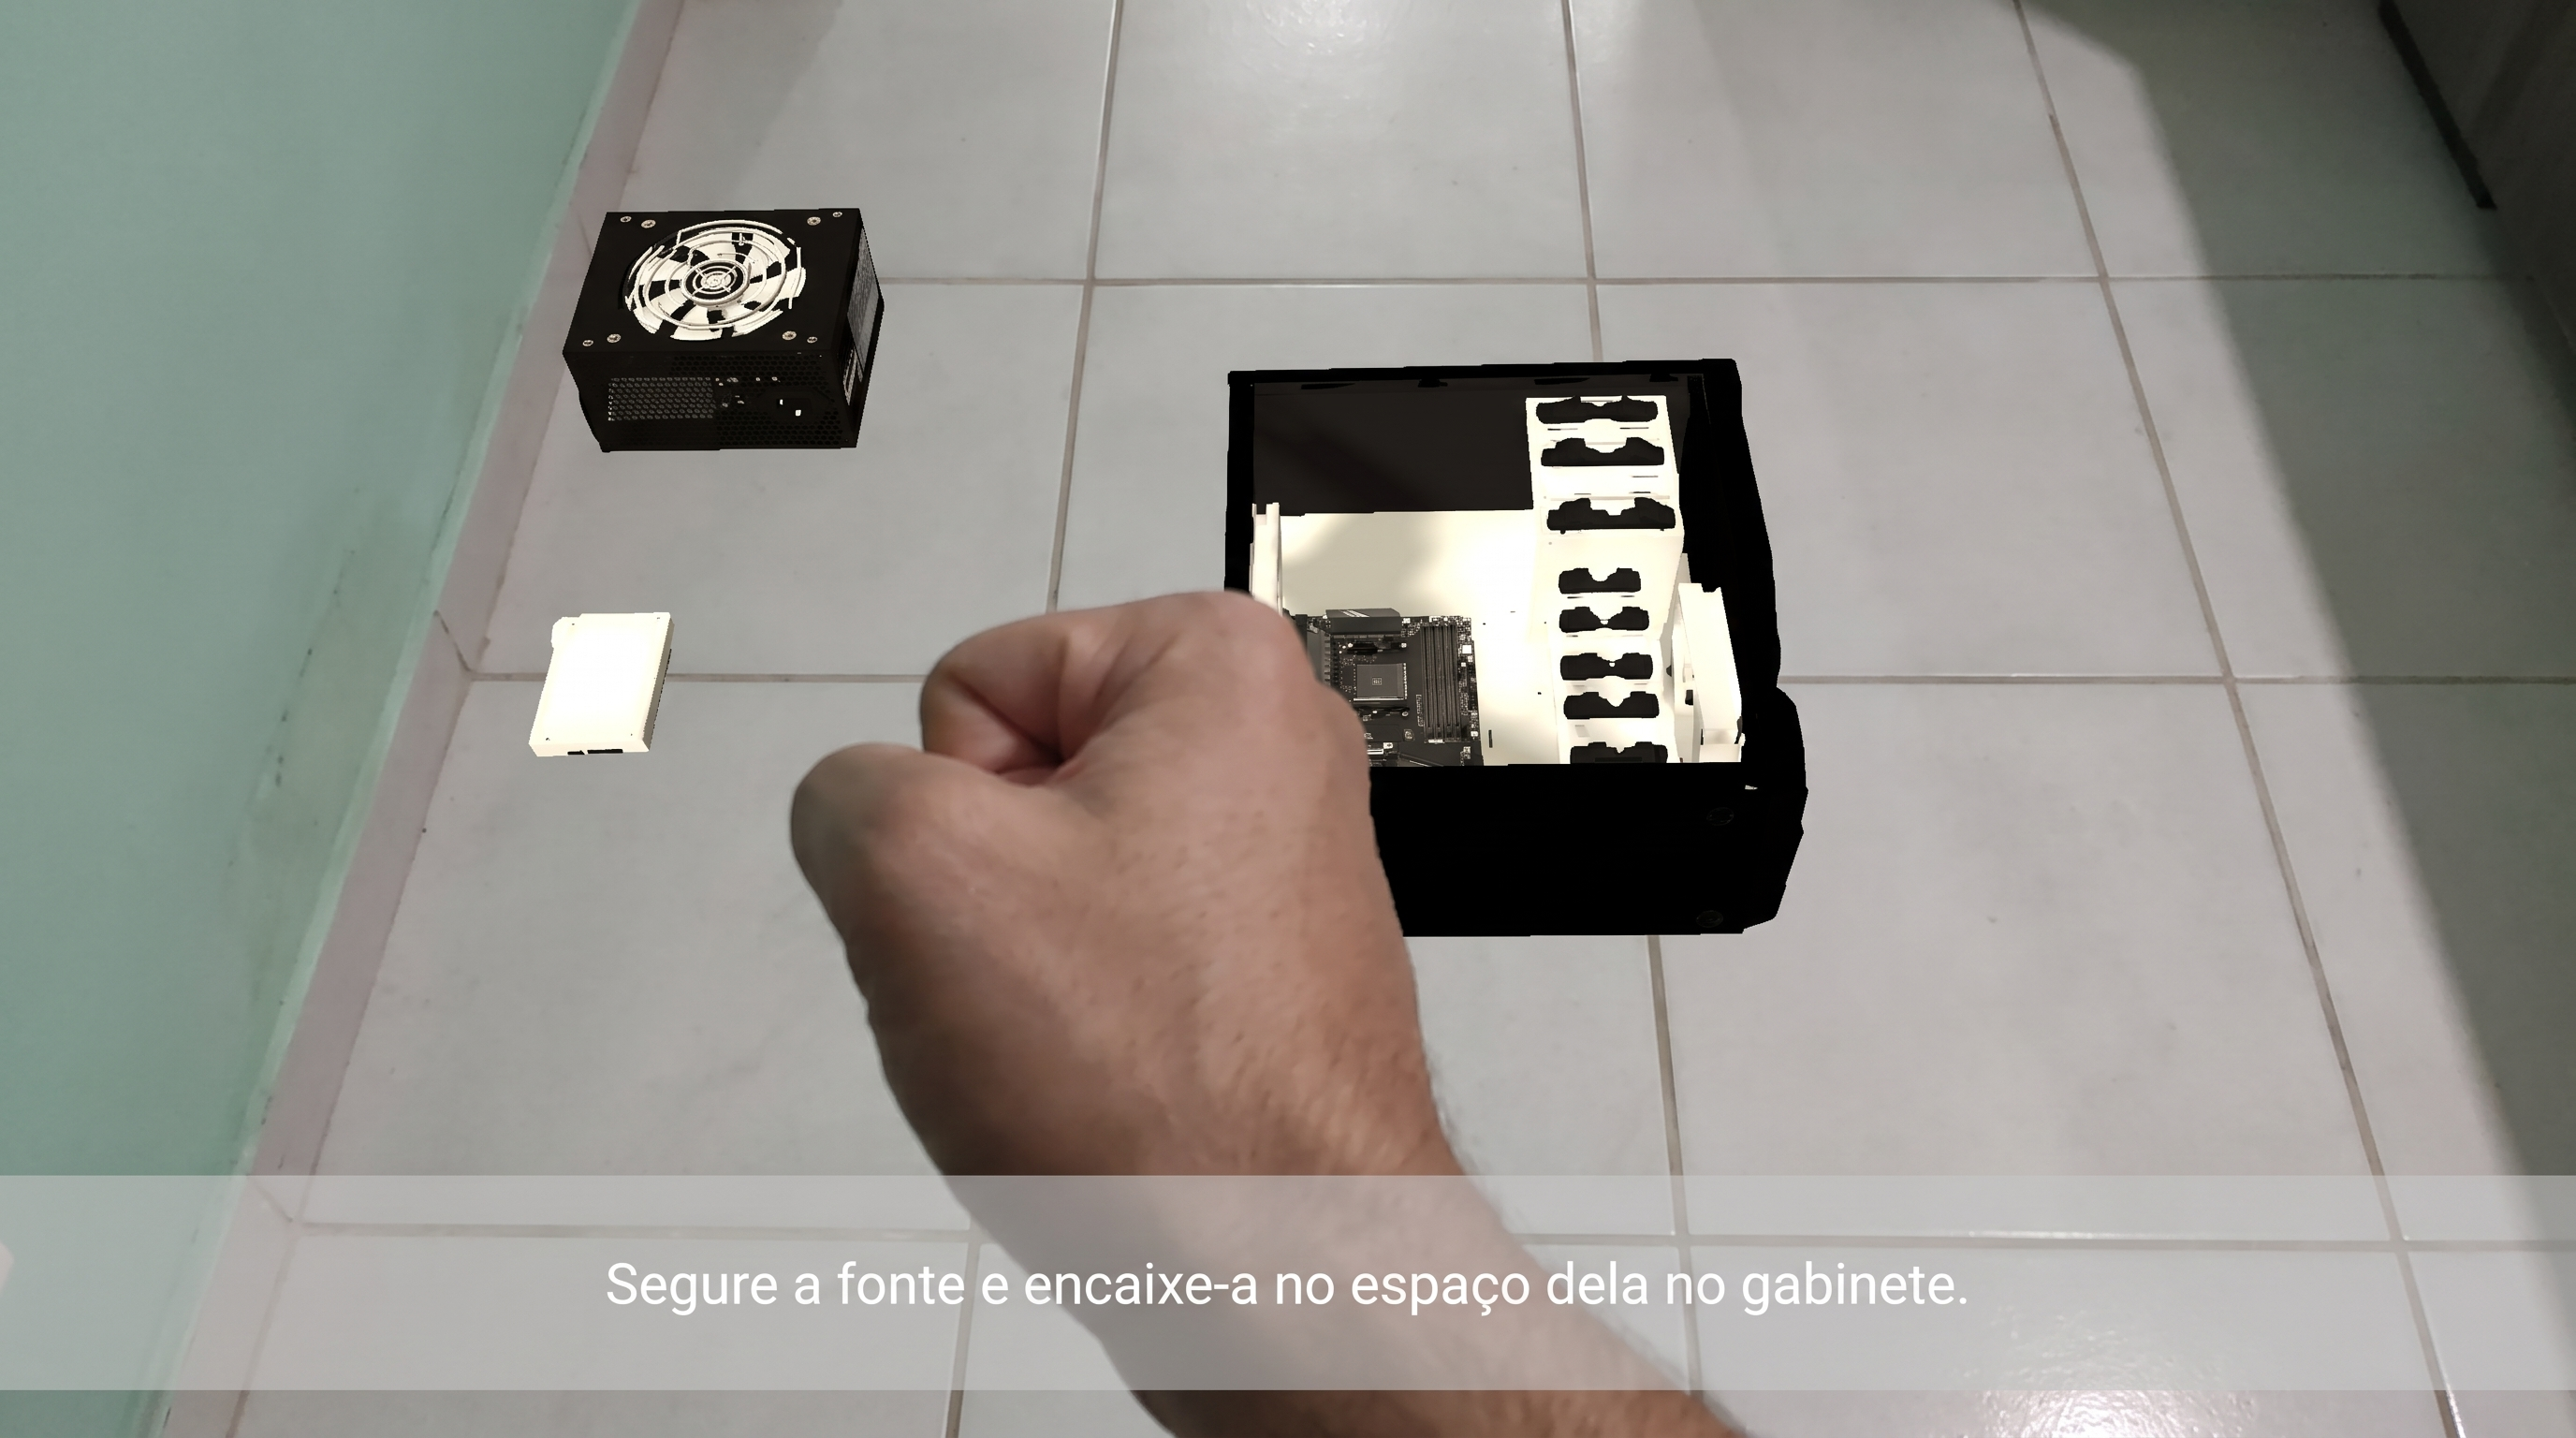
\includegraphics[width=\textwidth]{imgs/savit-manipulacao-gestos.jpg}
    \caption{Interação por gestos (MediaPipe - Mão Fechada).}
    \label{fig:app-gestos}
\end{subfigure}
\hfill
\begin{subfigure}[t]{0.48\textwidth}
    \centering
    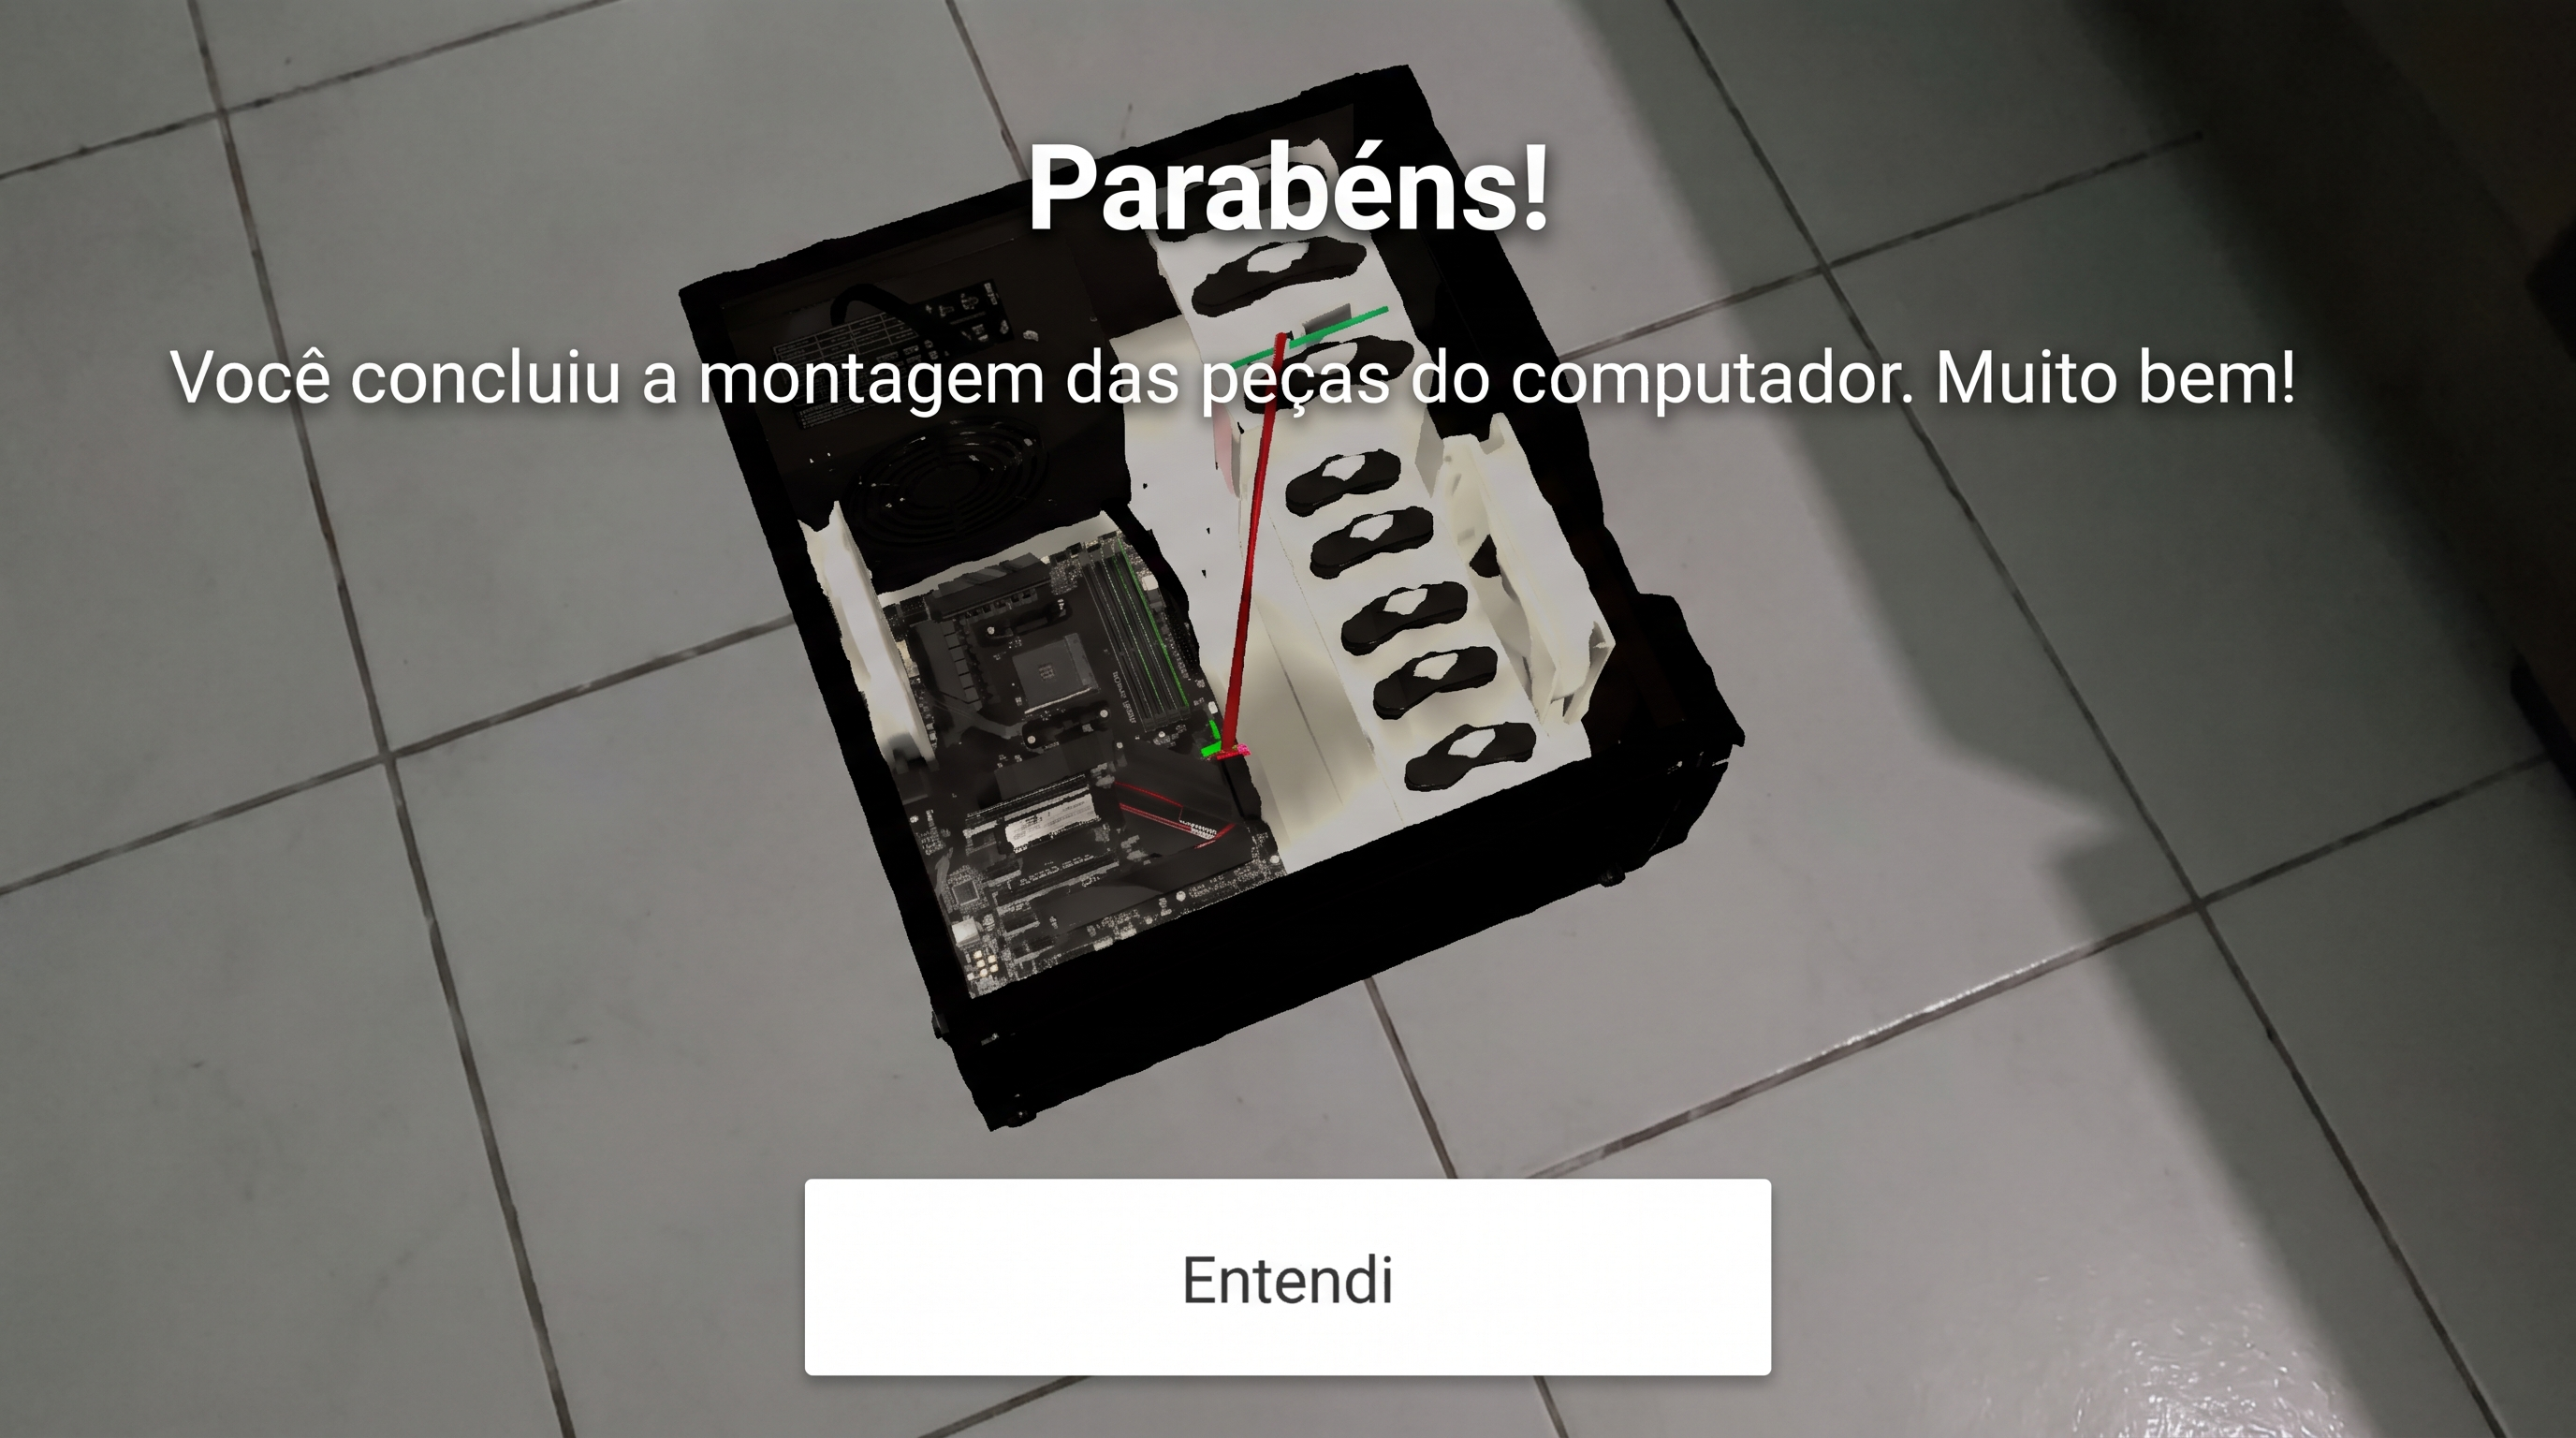
\includegraphics[width=\textwidth]{imgs/savit-encaixe-componentes.jpg}
    \caption{Validação e conclusão da montagem.}
    \label{fig:app-encaixe}
\end{subfigure}
\caption{Mecânicas de interação por gestos e confirmação de encaixe dos componentes.}
\end{figure}

\begin{figure}[H]
\centering
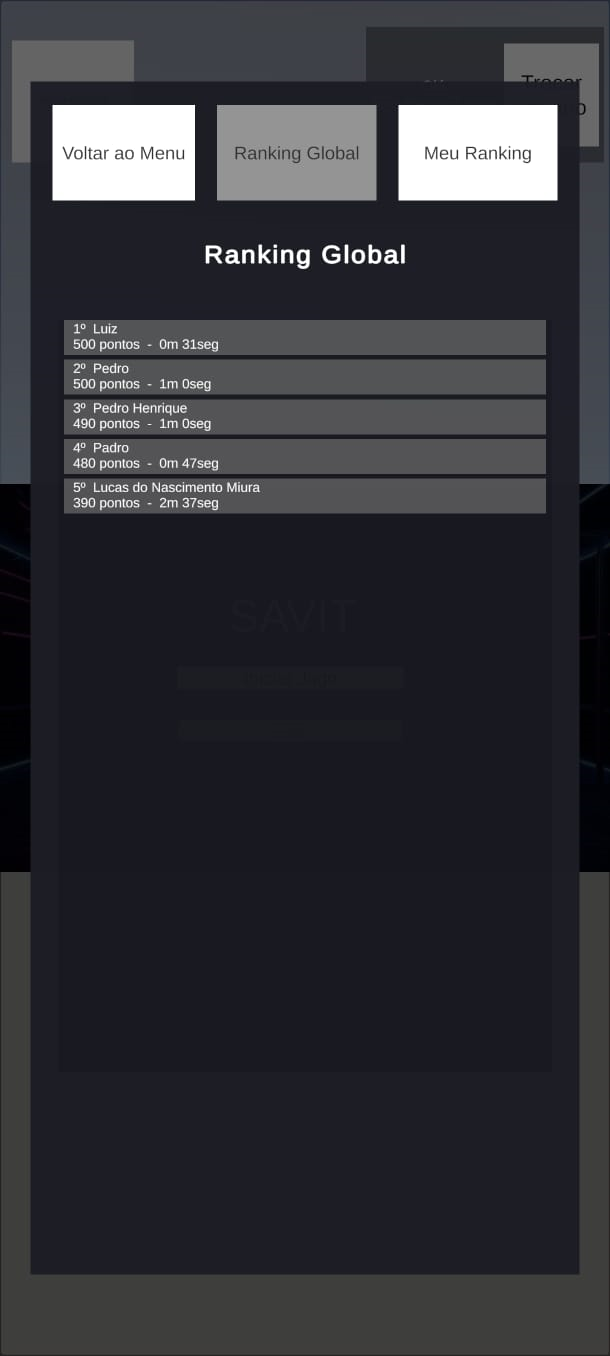
\includegraphics[width=0.45\textwidth]{imgs/ranking_global_app.png}
\caption{Visualização do Ranking Global na aplicação Android.}
\label{fig:app-ranking}
\end{figure}

\section{Diagramas UML: Modelagem do Sistema}
Representações diagramáticas de acordo com o paradigma da modelagem visual orientada a objetos (UML).

\subsection{Diagrama de casos de uso}
O diagrama de casos de uso foca nas interações entre o usuário, as funcionalidades de montagem por gestos e as respostas de ranking e backend.

\begin{figure}[H]
\centering
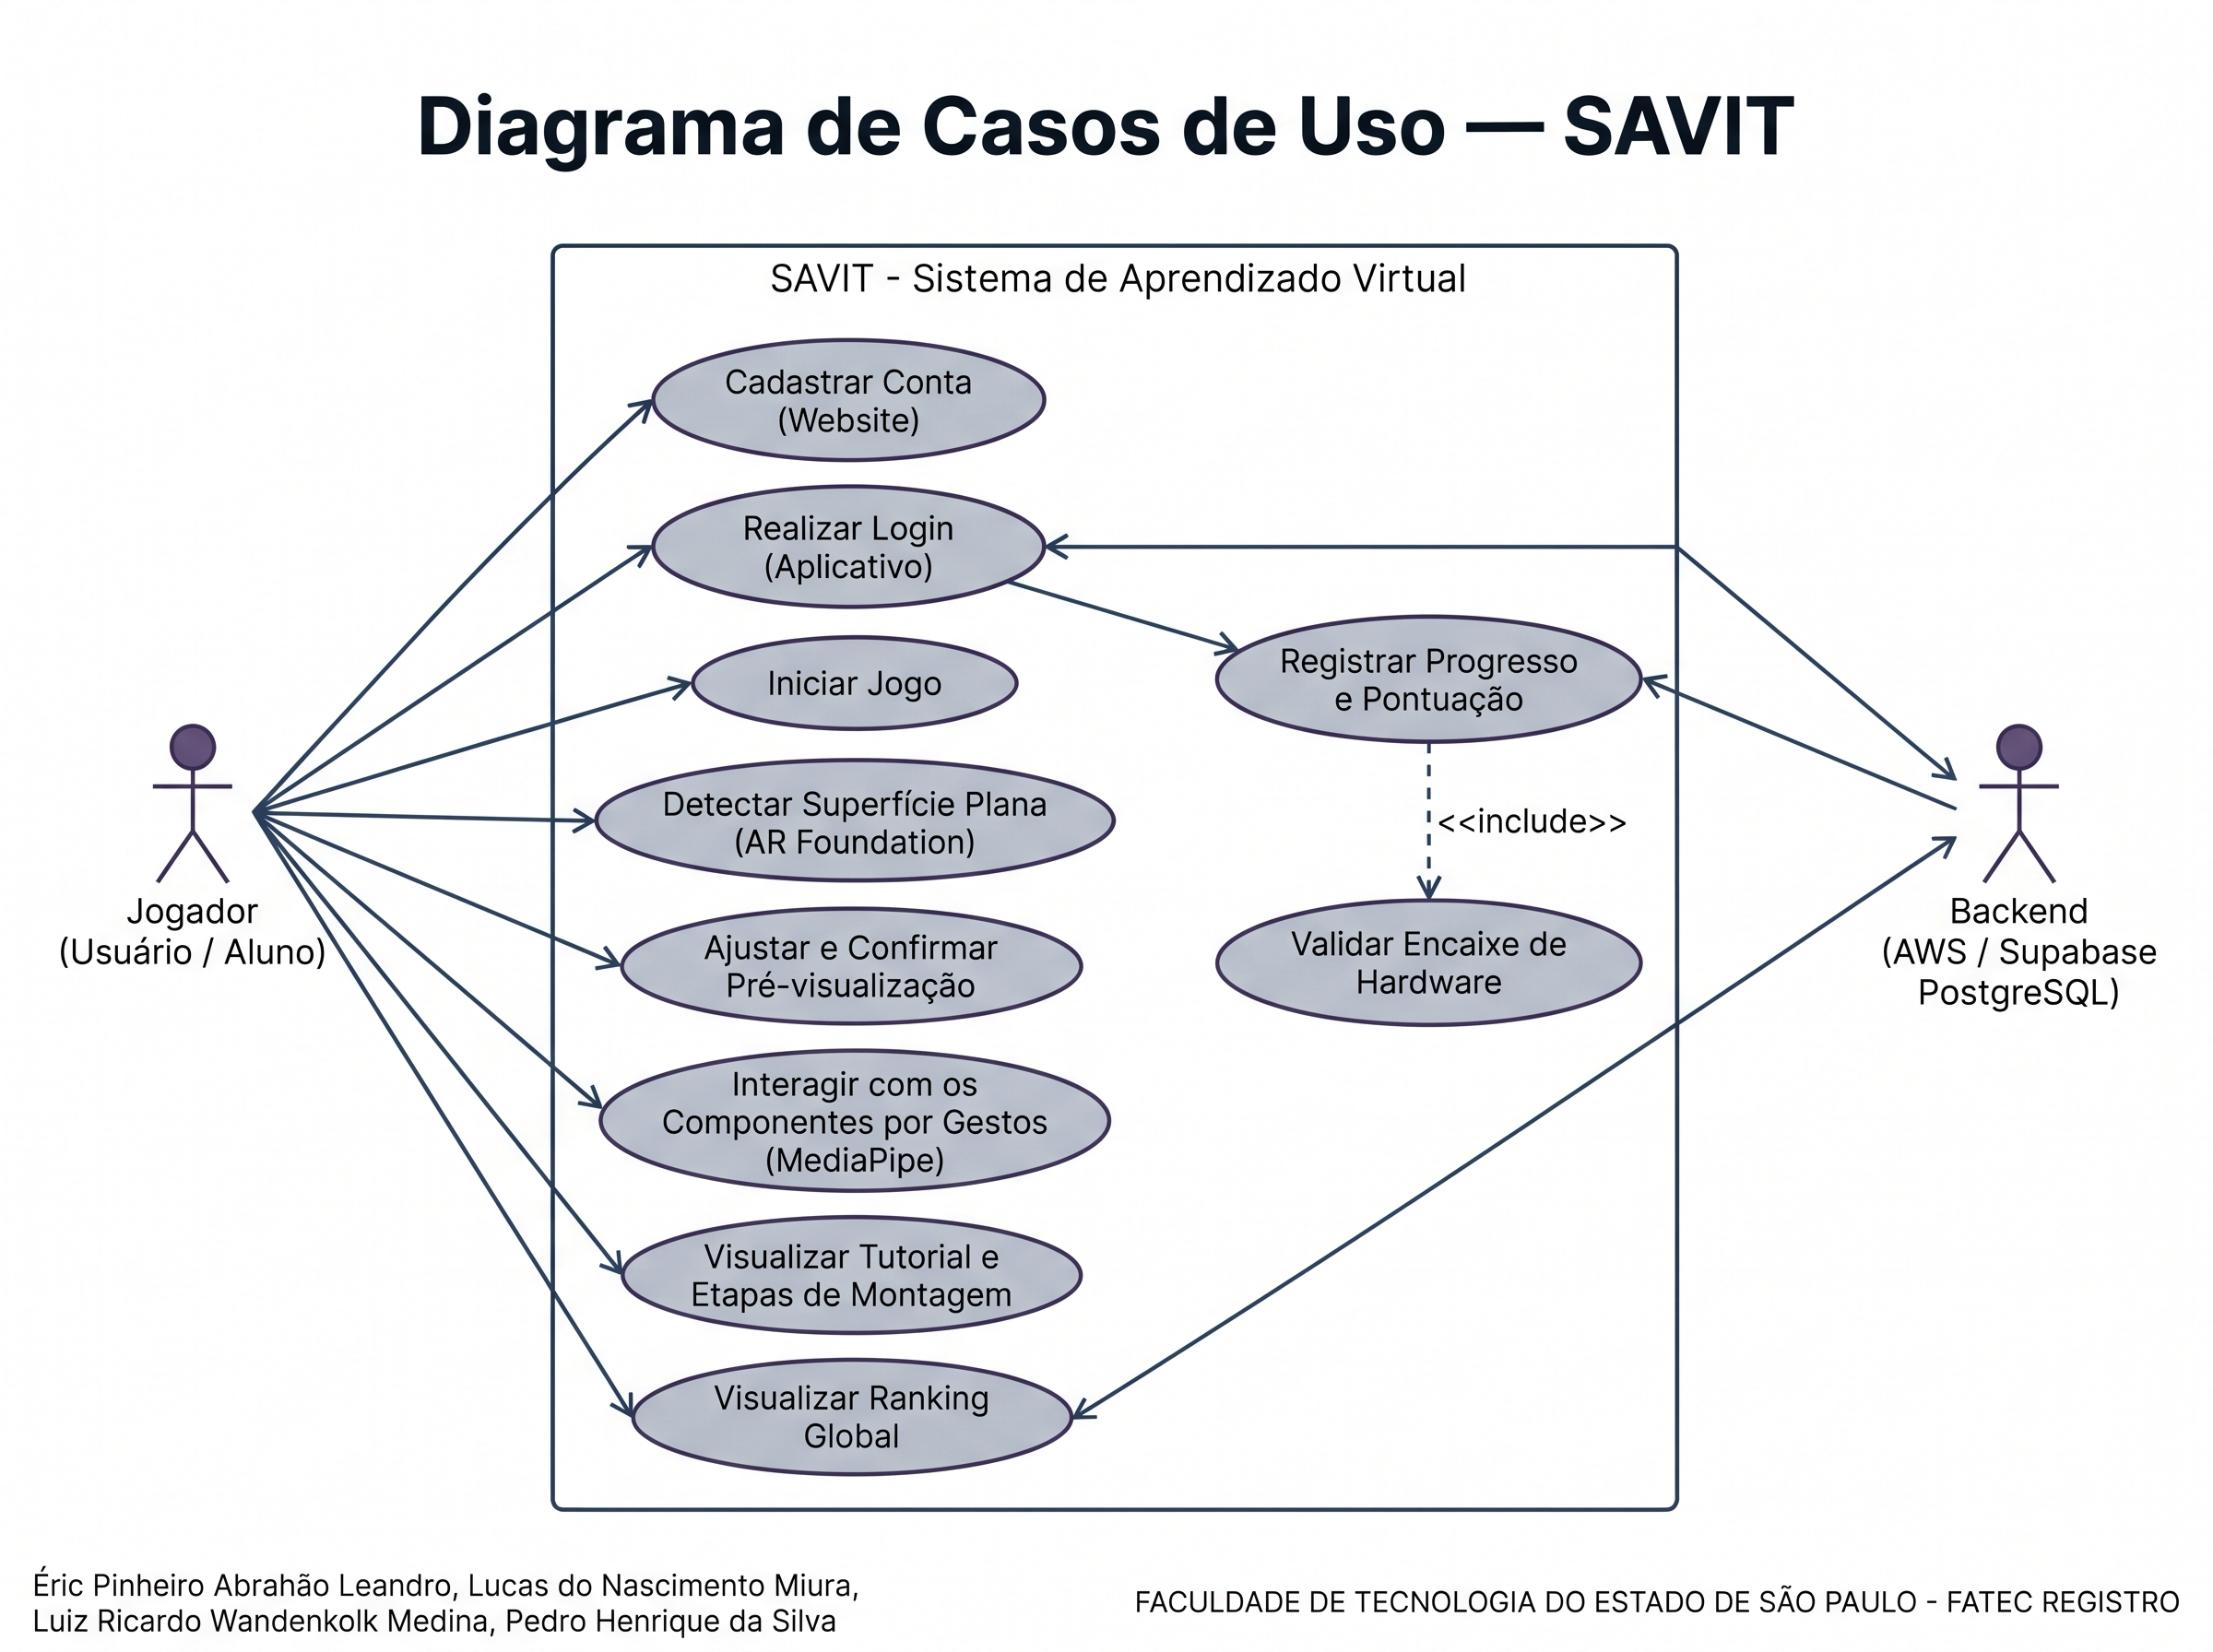
\includegraphics[width=0.9\textwidth]{imgs/uml-casos-de-uso.png}
\caption{Diagrama de casos de uso do projeto.}
\label{fig:casos-uso}
\end{figure}

\subsection{Diagrama de classes}
O diagrama de classes detalha a estrutura de C\# ativa, dividida por módulos de Realidade Aumentada, Interação, Tutoriais e Autenticação.

\begin{figure}[H]
\centering
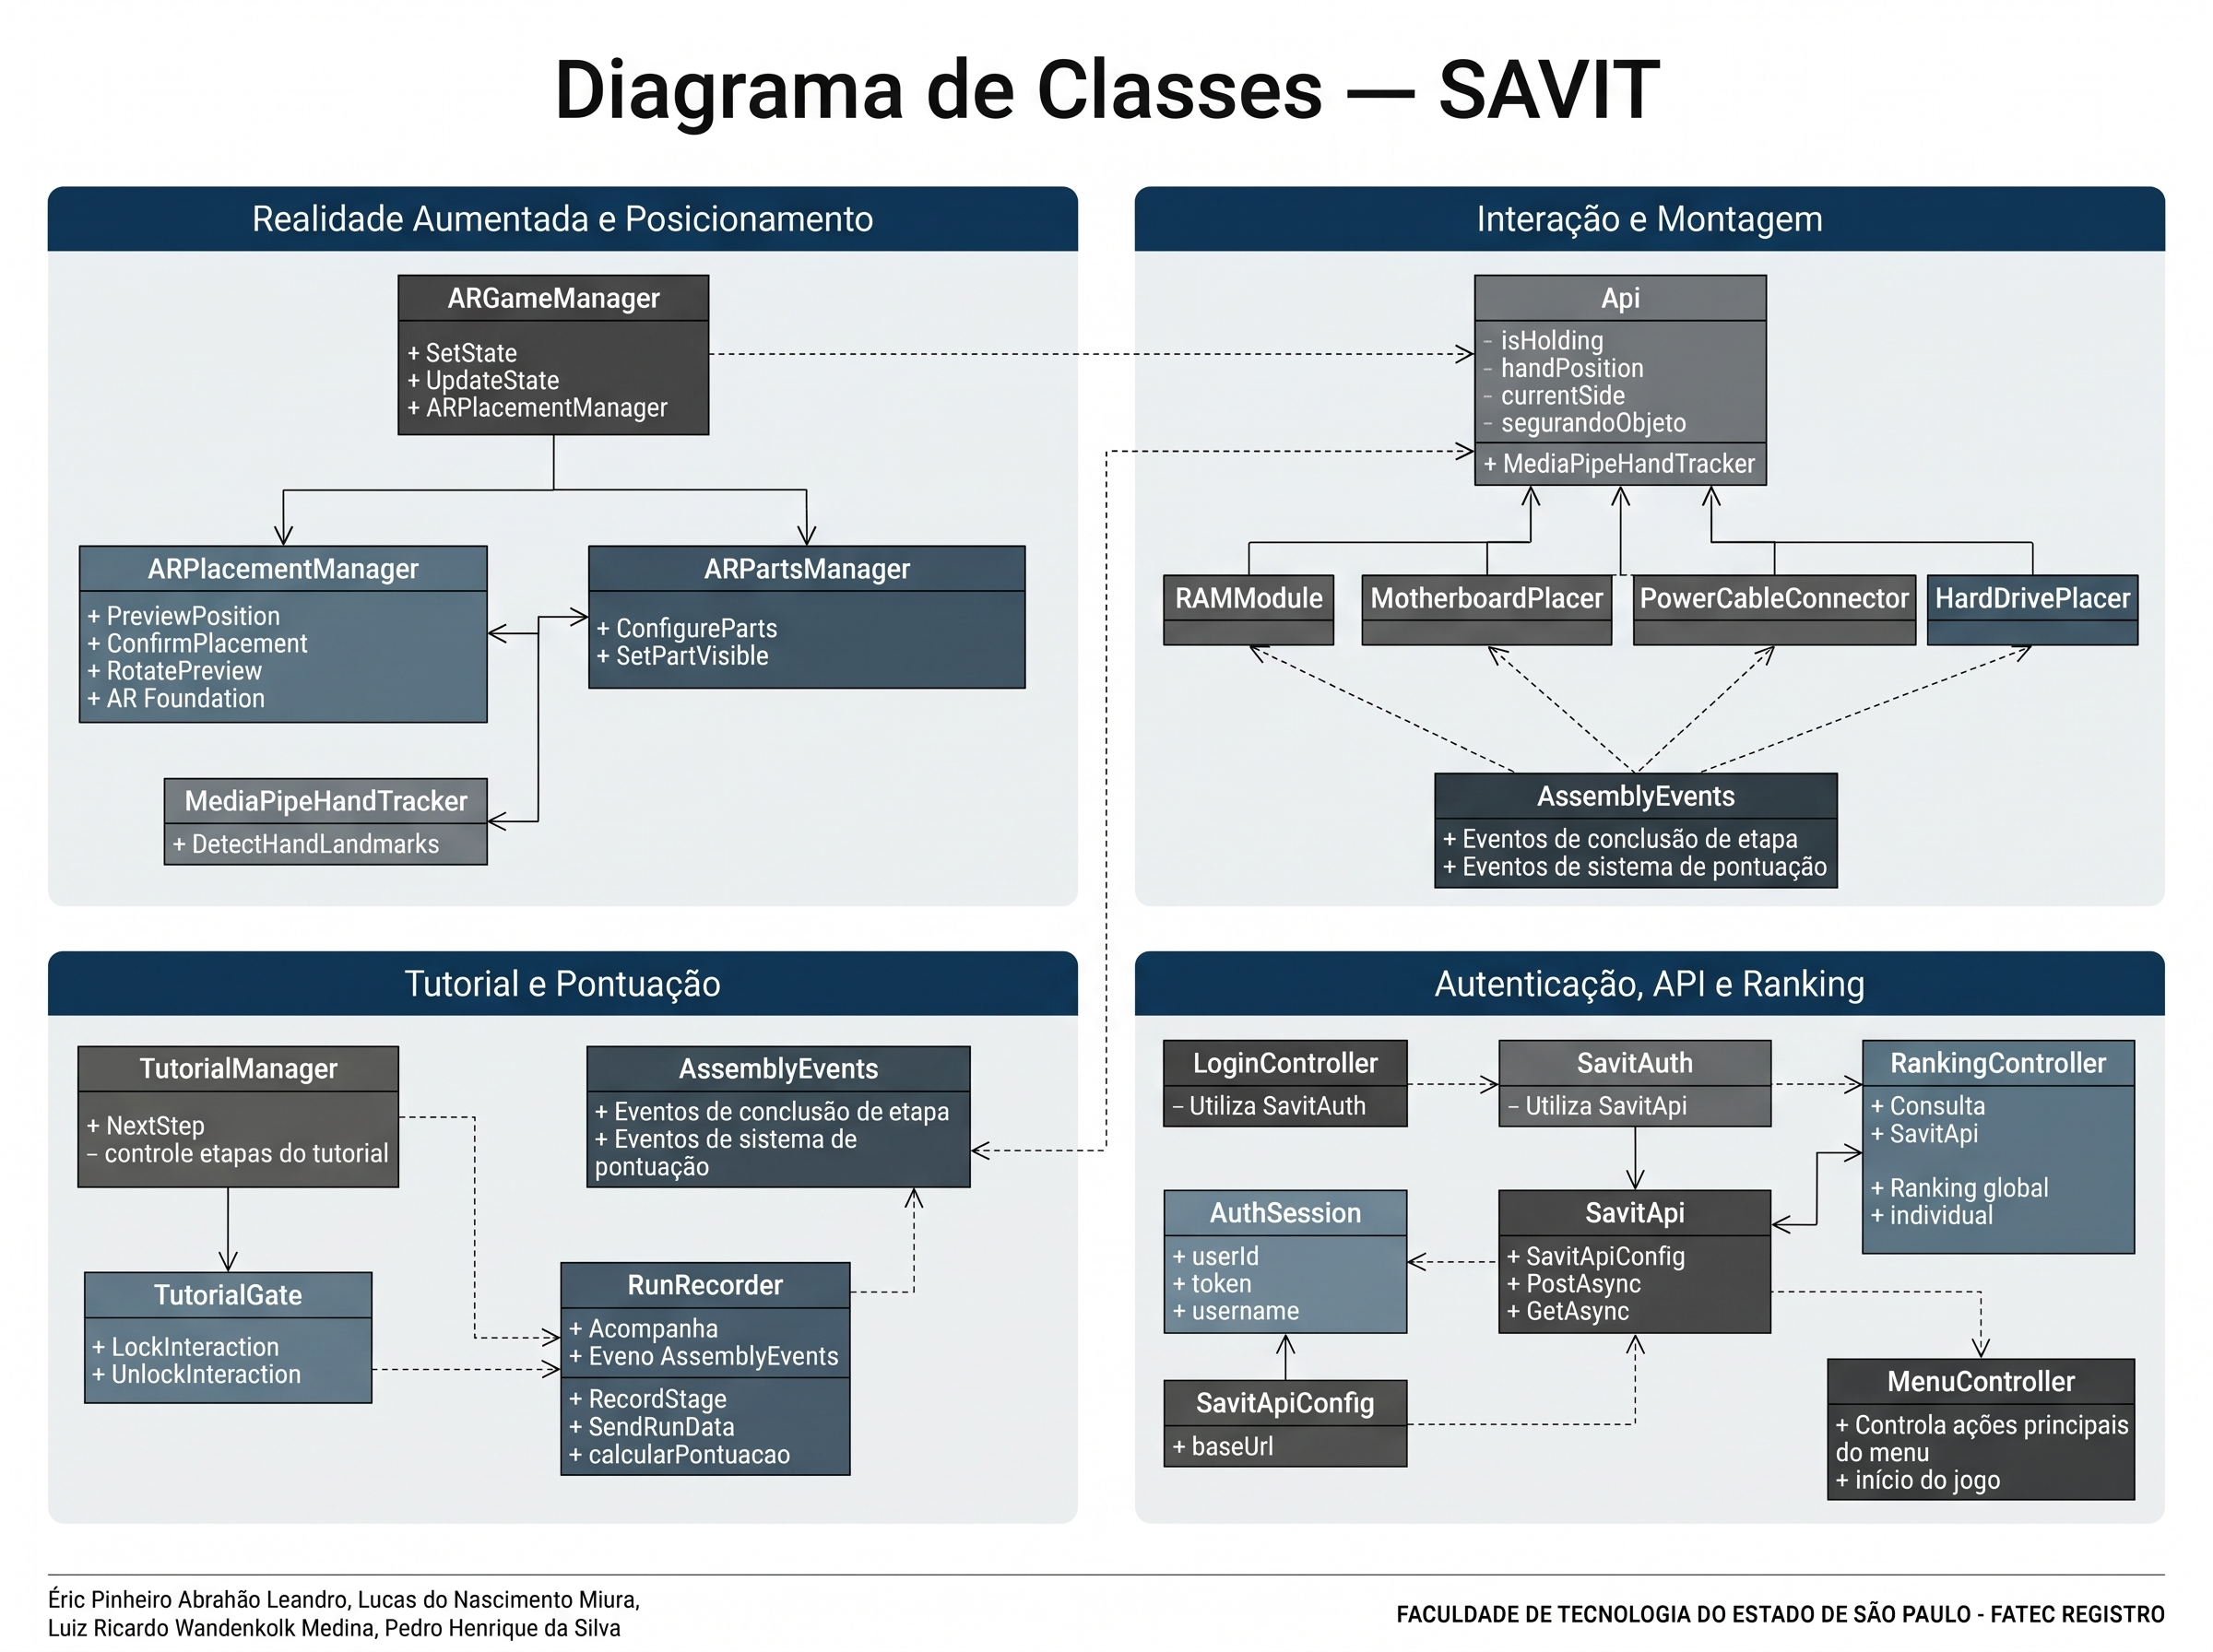
\includegraphics[width=\textwidth]{imgs/uml-classes.png}
\caption{Diagrama de classes do sistema SAVIT.}
\label{fig:classes}
\end{figure}

\subsection{Diagrama de objetos}
O diagrama de objetos ilustra instâncias ativas do sistema durante uma partida de montagem prática.

\begin{figure}[H]
\centering
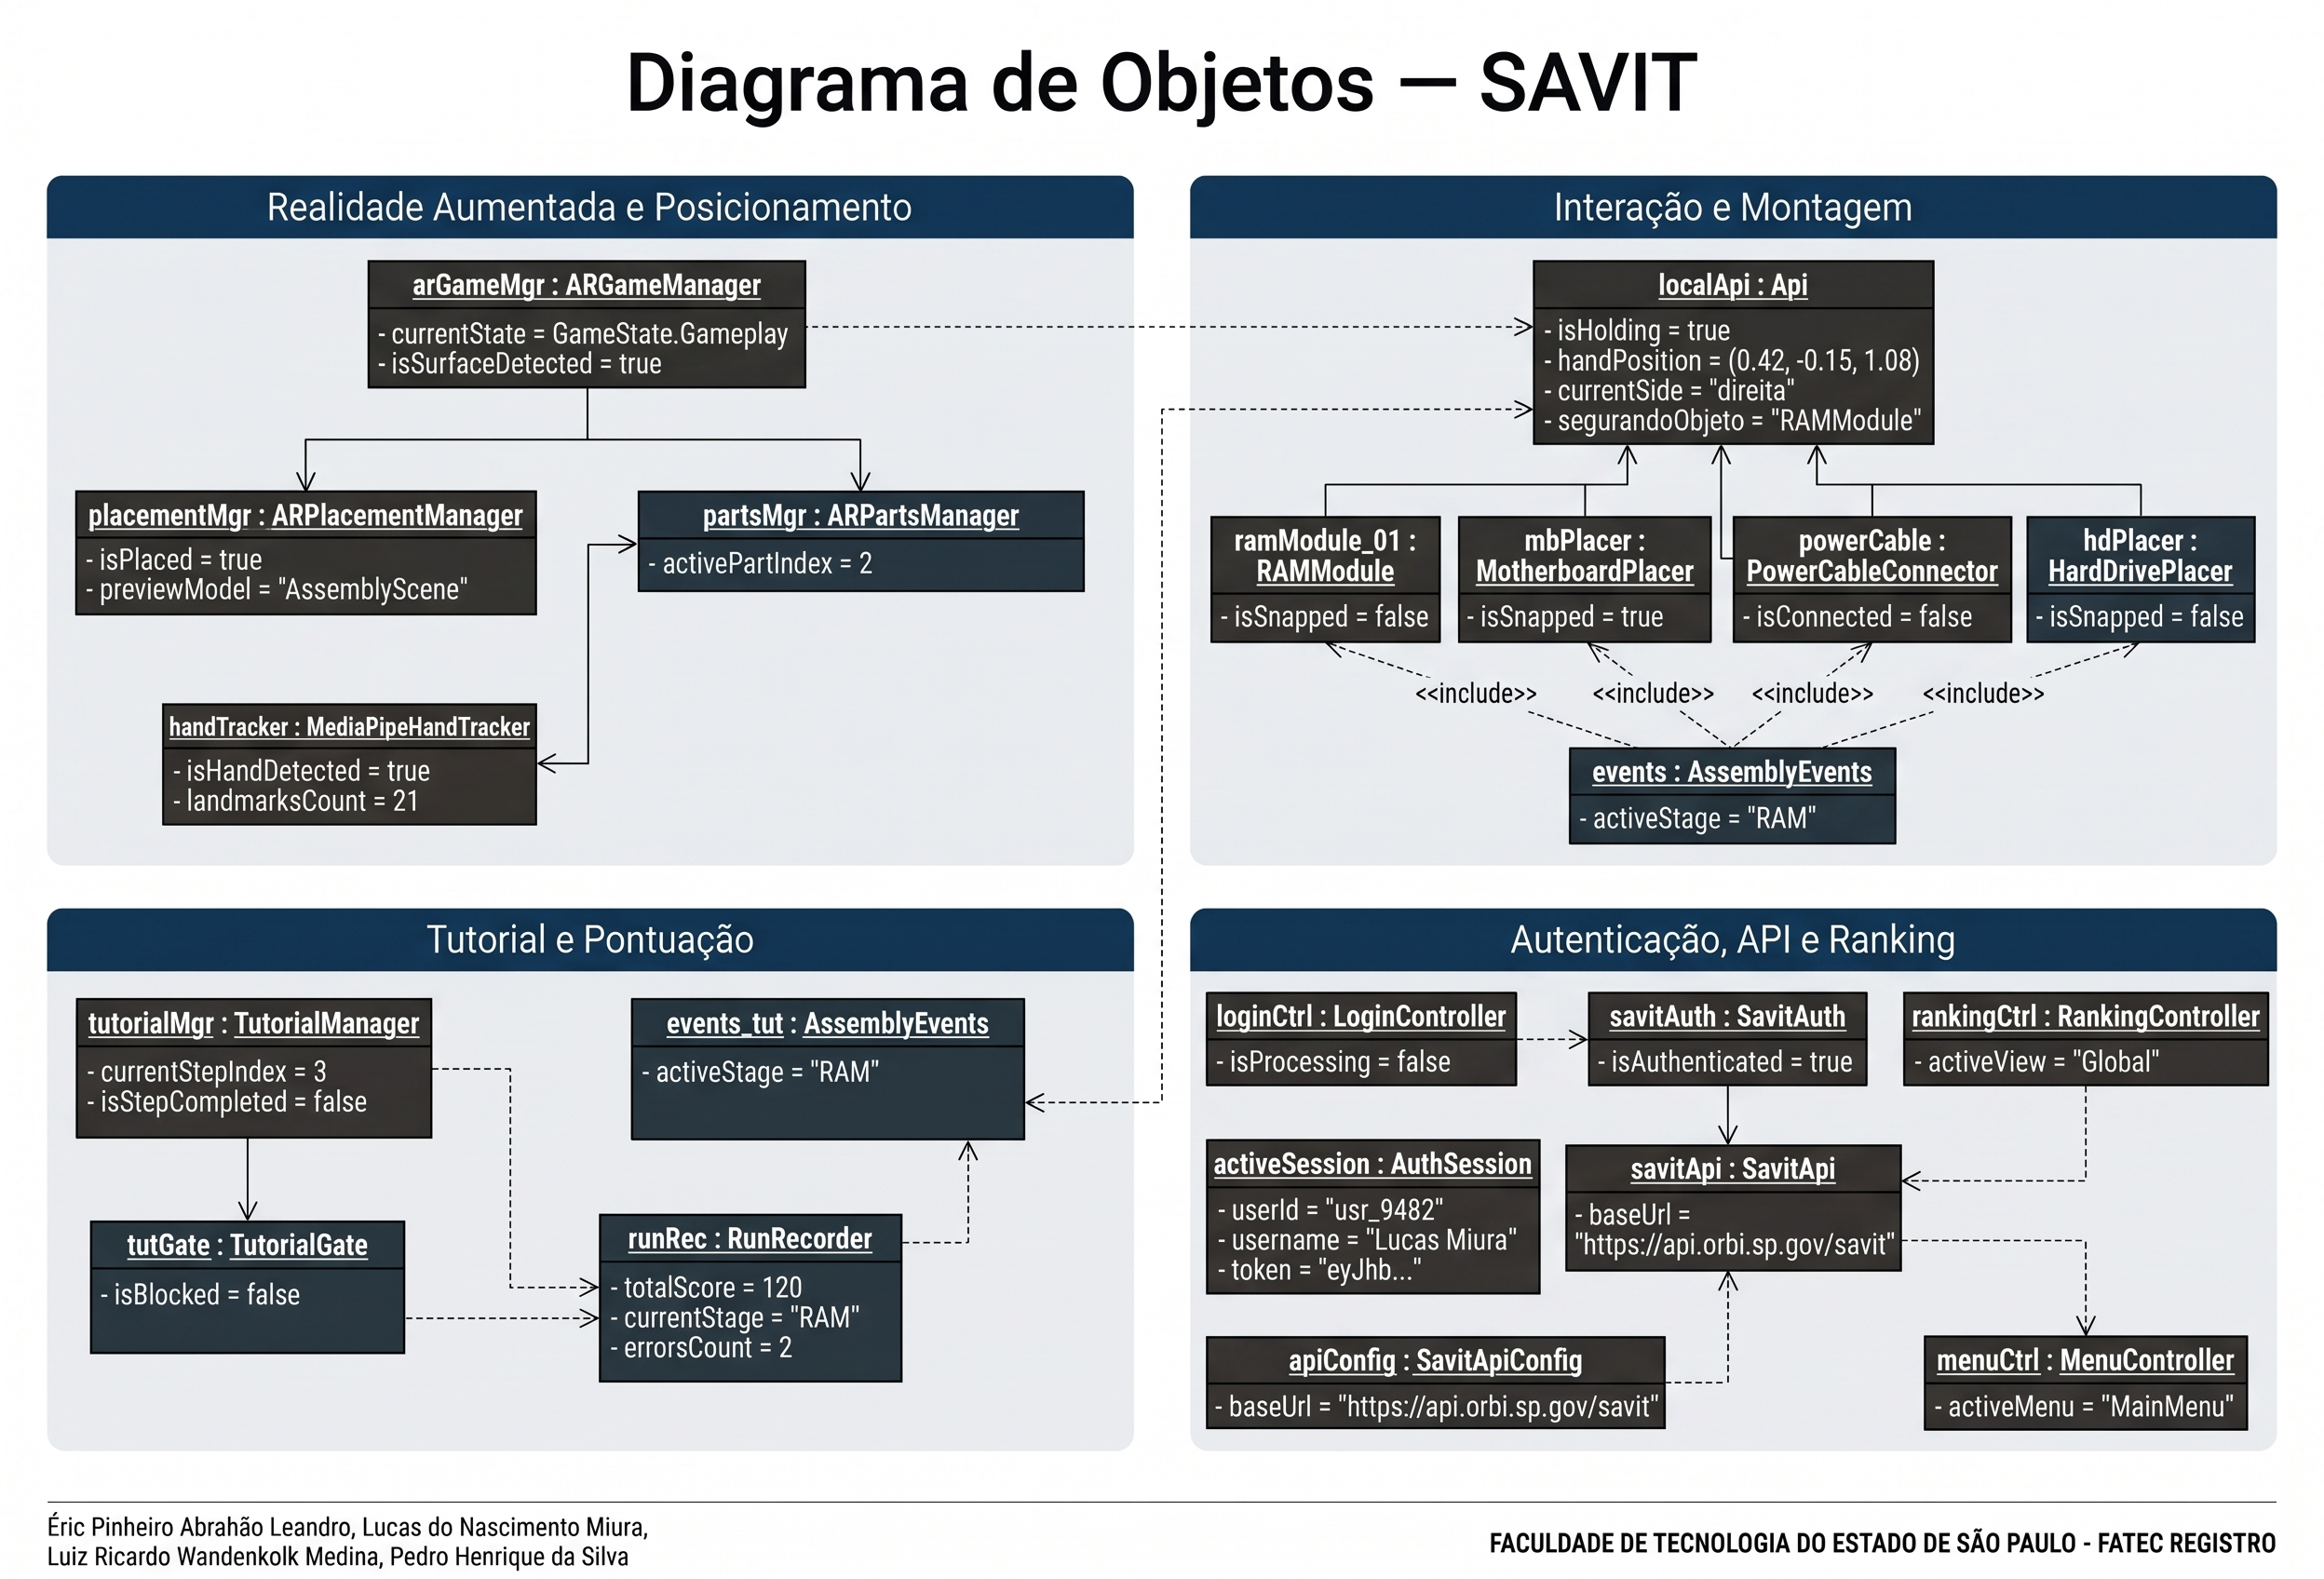
\includegraphics[width=\textwidth]{imgs/uml-objetos.png}
\caption{Diagrama de objetos do sistema.}
\label{fig:objetos}
\end{figure}

\section{Modelagem do Banco de Dados}
O SAVIT utiliza o PostgreSQL no Supabase.

\subsection{Diagrama lógico}
Identificação lógica e conceitual das tabelas e relacionamentos.

\begin{figure}[H]
\centering
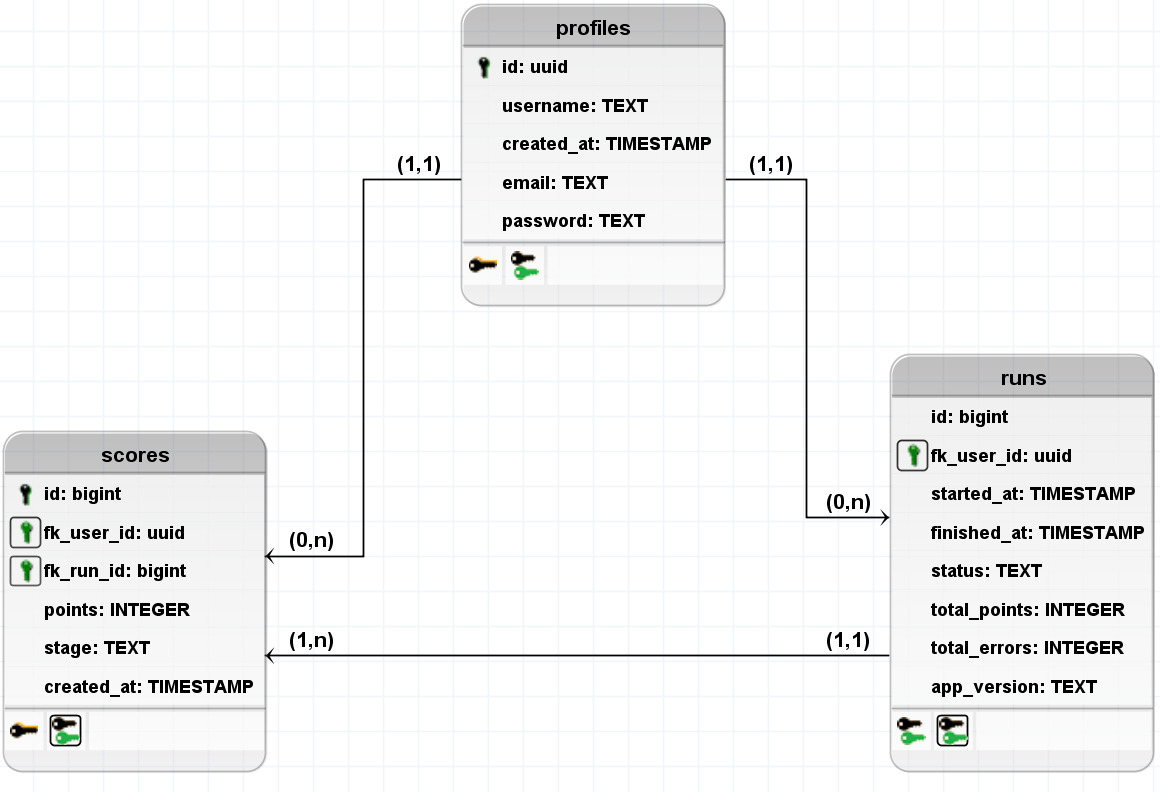
\includegraphics[width=0.85\textwidth]{imgs/diagrama_logico.png}
\caption{Diagrama lógico de dados do banco de dados.}
\label{fig:diag-logico}
\end{figure}

\subsection{Diagrama relacional}
Estrutura física de tabelas, chaves e integridade relacional.

\begin{figure}[H]
\centering
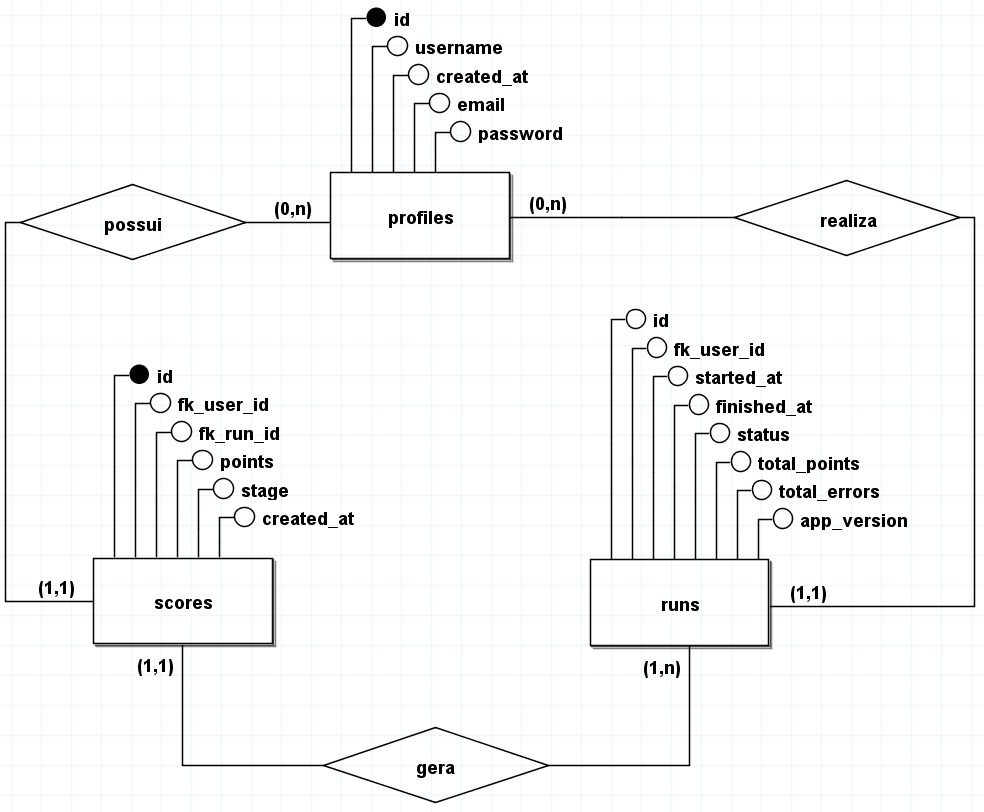
\includegraphics[width=0.85\textwidth]{imgs/diagrama_relacional.png}
\caption{Diagrama relacional (DER) do banco de dados.}
\label{fig:diag-relacional}
\end{figure}

\section{DevOps e Infraestrutura}
A infraestrutura em nuvem garante escalabilidade por meio da arquitetura sem servidor (serverless) da AWS aliada ao Supabase.

\subsection{Arquitetura e Integração Geral (DevOps)}
Detalhamento de ambientes, esteiras de build e o processamento local.

\begin{figure}[H]
\centering
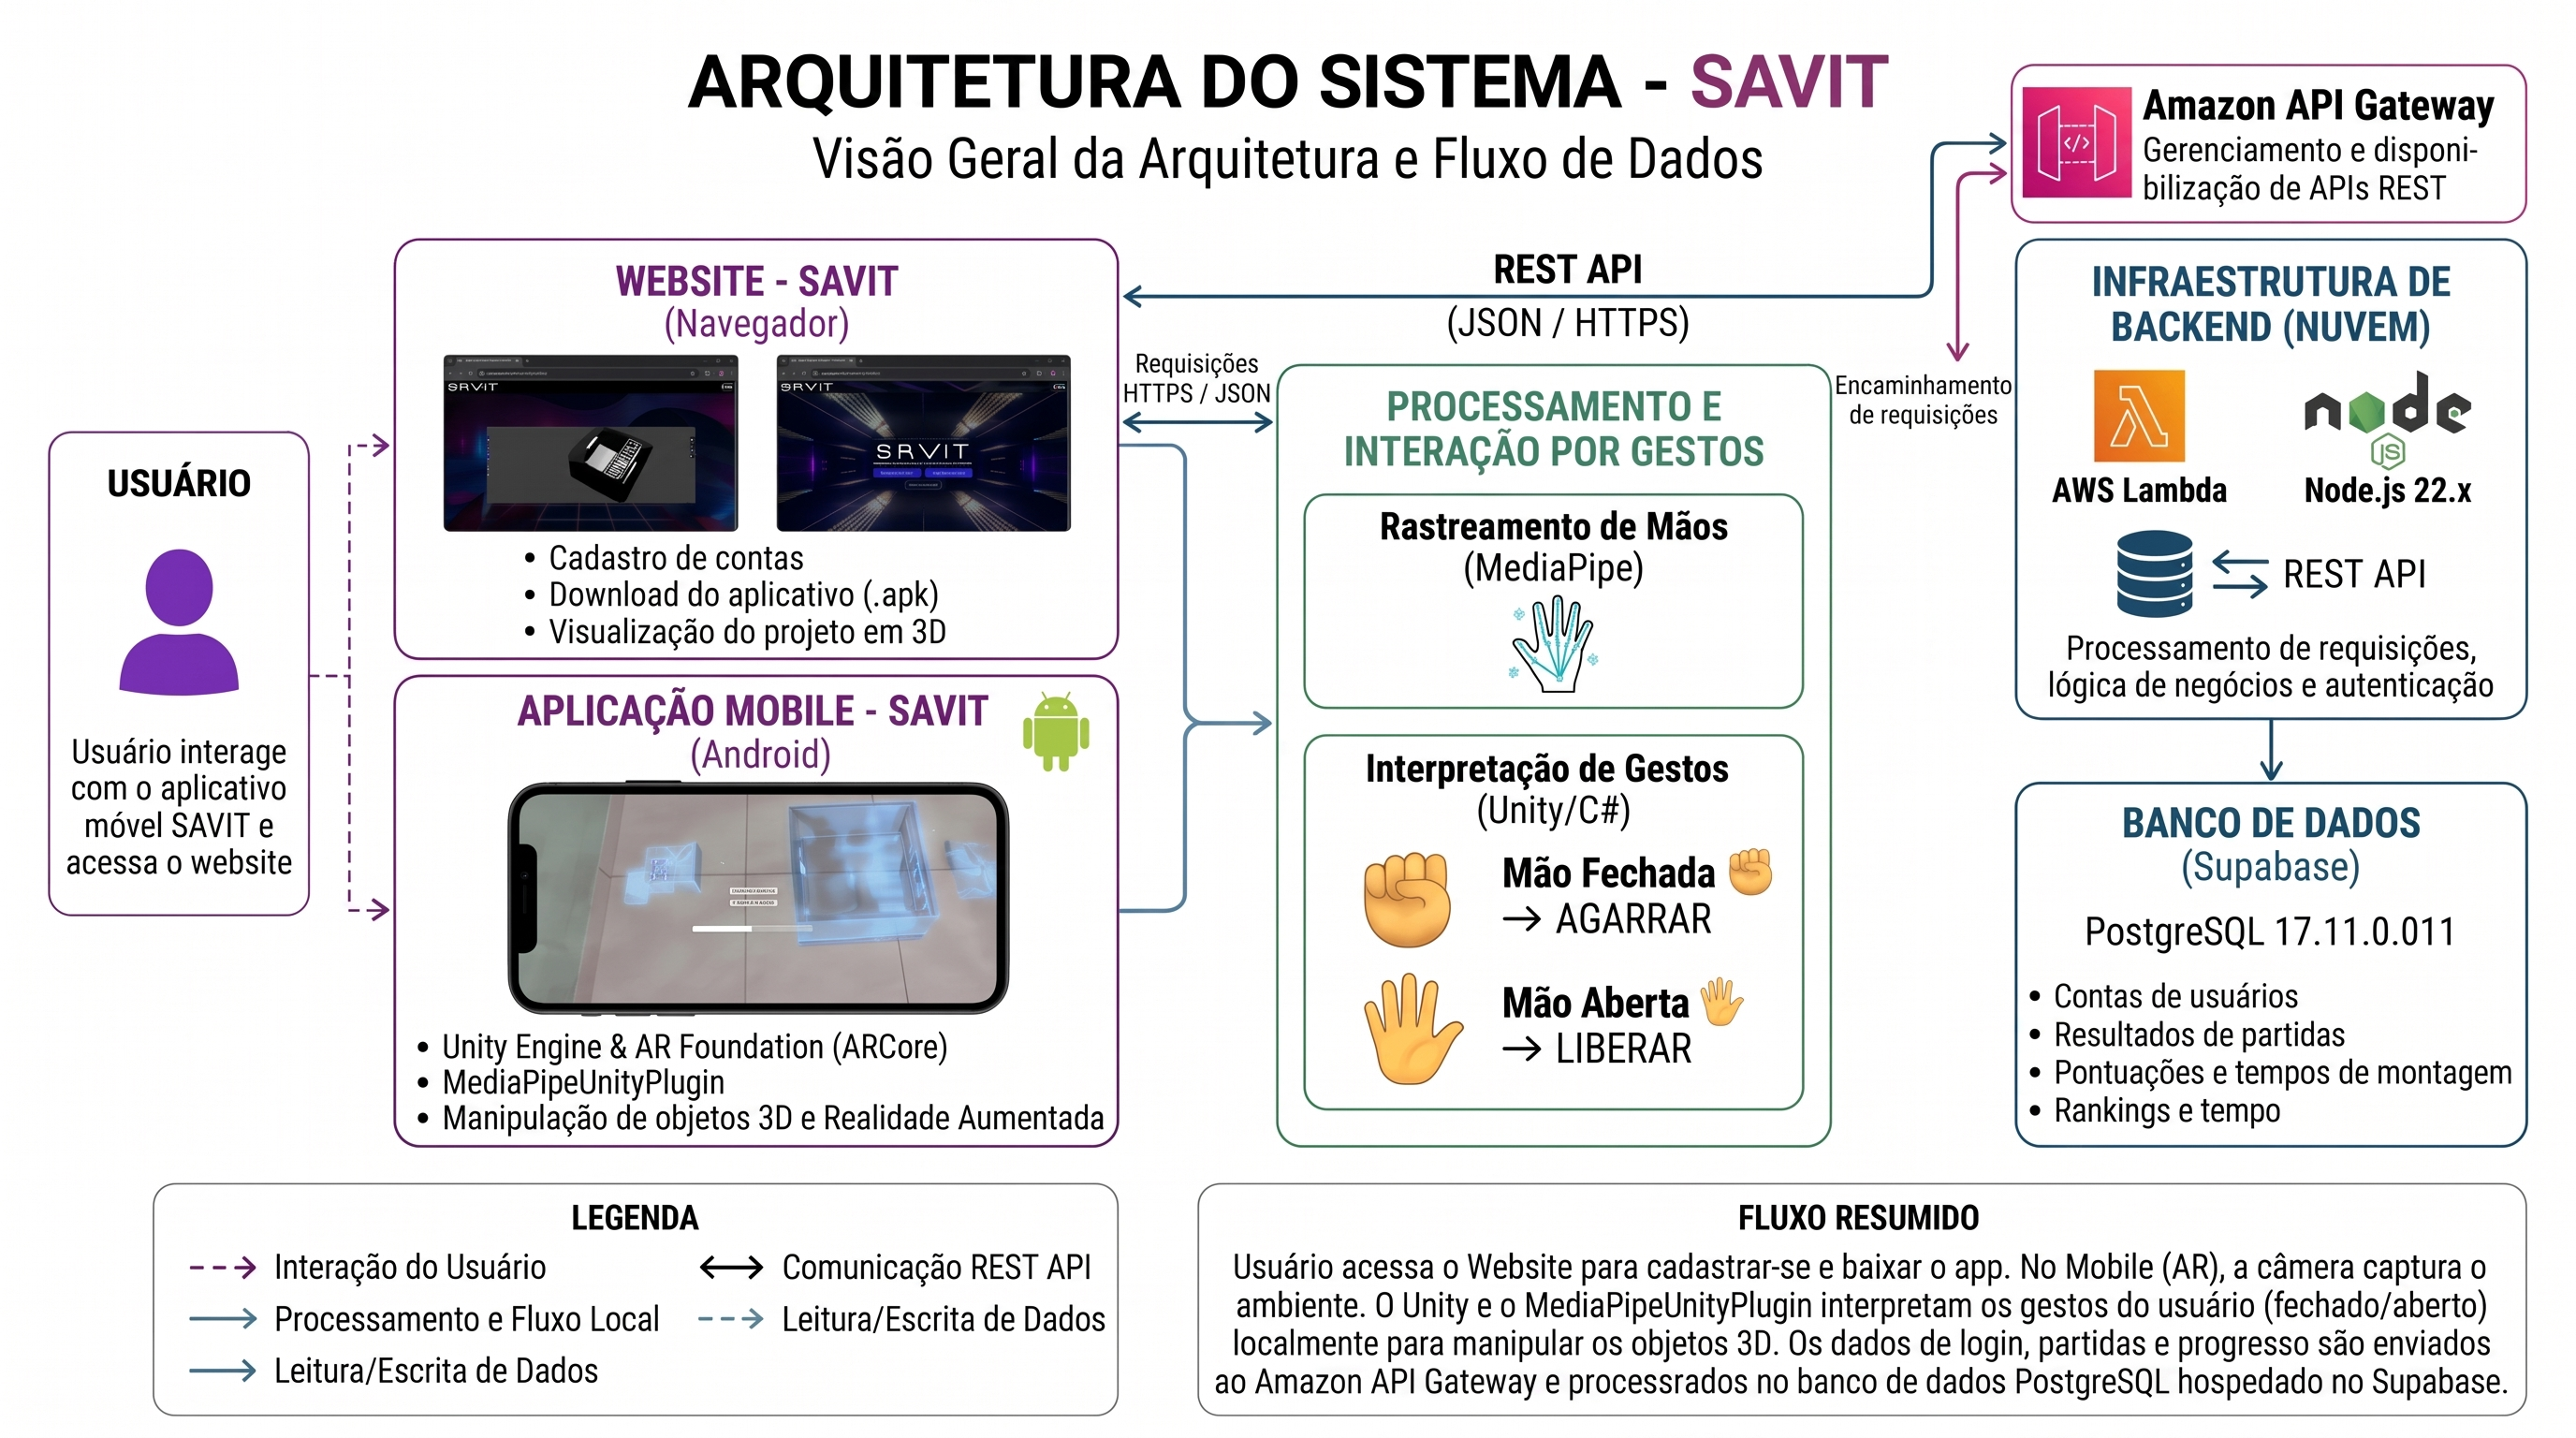
\includegraphics[width=0.9\textwidth]{imgs/devops-infraestrutura.png}
\caption{Visão geral da arquitetura de DevOps.}
\label{fig:devops}
\end{figure}

\subsection{Infraestrutura de Rede}
O diagrama lógico da rede mapeia a ausência de conexões diretas entre clientes e bancos, assegurando a segurança intermediada pelo API Gateway e Lambda.

\begin{figure}[H]
\centering
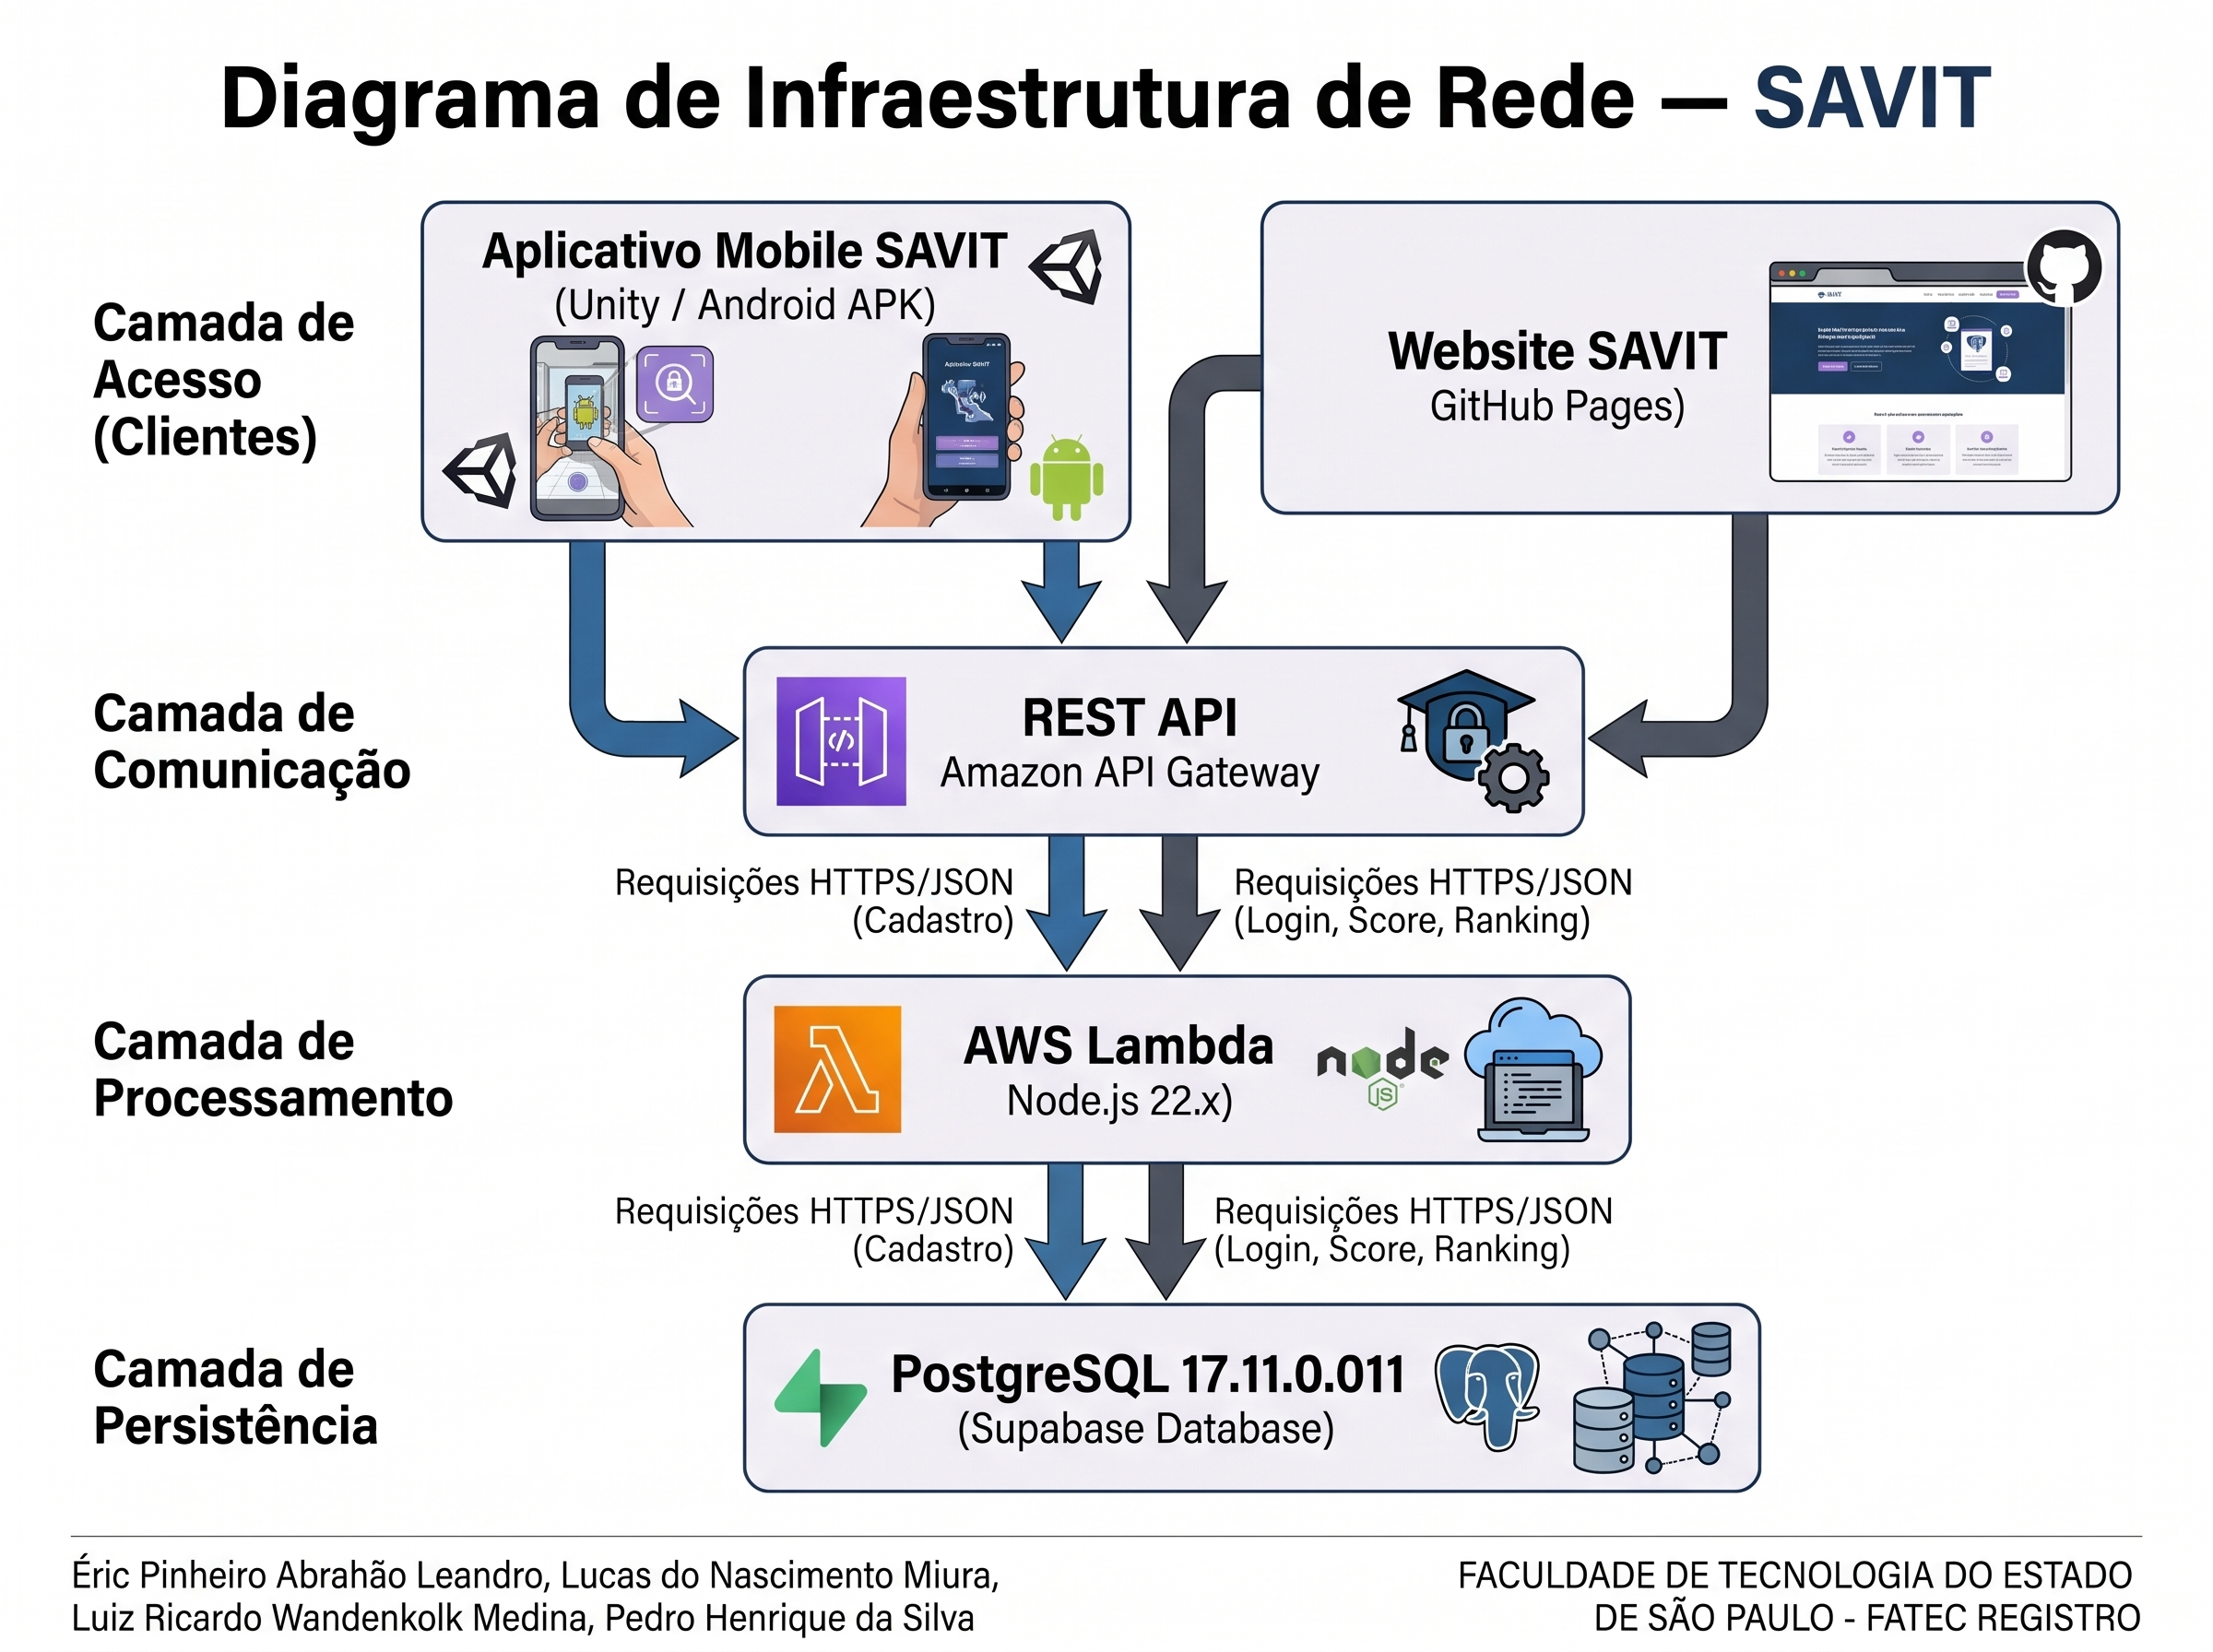
\includegraphics[width=0.9\textwidth]{imgs/diagrama-infraestrutura-rede.png}
\caption{Diagrama de Infraestrutura de Rede do SAVIT.}
\label{fig:rede}
\end{figure}

\section{Conclusão}
Este documento de artefatos acadêmicos consolida a especificação do SAVIT em todas as suas vertentes. Os novos diagramas retratam o escopo e o software em execução com total consistência.

\end{document}